% Chapter Template

\chapter{Αρχιτεκτονική Συστήματος} % Main chapter title

\label{Chapter4}
Στο παρόν κεφάλαιο θα παρουσιαστεί η αρχιτεκτονική του συστήματος που υλοποιήθηκε, το λογισμικό και τα επιμέρους εργαλεία που χρησιμοποιήθηκαν, με στόχο την αυτόνομη ή μη λειτουργία της ρομποτικής πλατφόρμας Monstertruck. Επίσης, παρουσιάζονται και τα περιβάλλοντα προσομοίωσης του ρομπότ στις δύο και στις τρεις διαστάσεις, που χρησιμοποιήθηκαν κατά την υλοποίηση και την αποσφαλμάτωση του συστήματος.

%----------------------------------------------------------------------------------------
%	SECTION 1: ROS
%----------------------------------------------------------------------------------------
\section{Robotic Operating System} \label{sec:ros}
Οι περισσότερες ρομποτικές εφαρμογές απαιτούν ένα εξαιρετικά σύνθετο λογισμικό για να μπορούν να εκτελέσουν βασικές λειτουργίες, λογισμικό που μεγενθύνεται όσο εξελίσσεται το αντικείμενο της ρομποτικής και αυξάνουν οι απαιτήσεις της. Παράλληλα, κάθε ρομποτικό σύστημα παρουσιάζει ένα βαθμό ιδιαιτερότητας, λόγω διαφορετικού hardware, λογισμικού και σκοπού λειτουργίας, γεγονός που καθιστά την επαναχρησιμοποίηση κώδικα εξαιρετικά δύσκολο εγχείρημα. Επίσης, λόγω του μεγάλου μεγέθους του λογισμικού και των απαιτήσεων ταυτόχρονης λειτουργίας και επικοινωνίας μεταξύ των επιμέρους τμημάτων, από το επίπεδο των οδηγών (drivers) των επιμέρους συσκευών του ρομποτικού συστήματος μέχρι τα επίπεδα της αντίληψης, επεξεργασίας και λήψης αποφάσεων, καθίσταται απαραίτητη η ανάγκη για μία μέθοδο υψηλής κλίμακας ενσωμάτωσης λογισμικού.

\bigskip
Για την επίλυση των παραπάνω προβλημάτων και όχι μόνο, οι \citeauthor{ros} \cite{ros} ανέπτυξαν το ROS (Robot Operating System) \footnote{ROS Tutorials: \url{www.wiki.ros.org/ROS/StartGuide}, Mastering ROS for Robotics Programming \cite{mastering_ros}} . Το ROS αποτελεί ένα ευέλικτο framework ρομποτικής που προσφέρει ένα σύνολο εργαλείων και βιβλιοθηκών λογισμικού, ενώ παράλληλα επιβάλλει ένα σύνολο αυστηρών συμβάσεων, με στόχο την απλοποίηση της ανάπτυξης σύνθετων και εύρωστων εφαρμογών για πληθώρα ρομποτικών συστημάτων. Επίσης, το ROS σχεδιάστηκε από την αρχή με απώτερο στόχο την συνεργασία του κόσμου της ρομποτικής για την κατανεμημένη ανάπτυξη λογισμικού ανοικτού κώδικα για ρομποτικές εφαρμογές. Το ROS χαρακτηρίζεται, γενικά, ως:
\begin{itemize}
	\item \textbf{Peer-to-Peer}, καθώς ένα σύστημα βασισμένο στο ROS αποτελείται από ένα σύνολο διεργασιών που τρέχουν σε έναν ή περισσότερους hosts που συνδέονται μεταξύ τους μέσω μίας τοπολογίας Peer-to-Peer και μπορούν να επικοινωνούν μεταξύ τους διαμέσου της διεργασίας του ROS Master.
	\item \textbf{Πολύγλωσσο}, καθώς επιτρέπει την χρήση διαφορετικών γλωσσών προγραμματισμού (C++, python κλπ) για την ανάπτυξη εφαρμογών, που μπορούν να επικοινωνούν μεταξύ τους, μέσω μίας αυστηρά ορισμένης διεπαφής.
	\item \textbf{Βασισμένο σε εργαλεία}, καθώς χρησιμοποιείται μεγάλος αριθμός μικρών εργαλείων για την ανάπτυξη και λειτουργία των επιμέρους τμημάτων του συστήματος.
	\item \textbf{Λεπτό}, από την άποψη ότι η ανάπτυξη των αλγορίθμων πραγματοποιείται σε ανεξάρτητες βιβλιοθήκες, οι οποίες έπειτα μπορούν να χρησιμοποιηθούν σε ένα σύστημα βασισμένο στο ROS, μέσω μικρών προγραμμάτων που εξάγουν την λειτουργικότητα των εν λόγω βιβλιοθηκών μέσω του συστήματος διεπαφών του ROS.
	\item \textbf{Ανοικτού Κώδικα}, ιδιότητα απαραίτητη και κρίσιμη για την κατανόηση της λειτουργίας του, την επέκταση του, αλλά και την ανάπτυξη και αποσφαλμάτωση του λογισμικού ρομποτικών εφαρμογών σε όλα τα επίπεδα.
\end{itemize}

\bigskip
Ένα σύστημα βασισμένο στο ROS, αποτελείται από ένα σύνολο διεργασιών που ονομάζονται \textit{κόμβοι} (\textit{nodes}) και επικοινωνούν μεταξύ τους, θυμίζοντας τοπολογικά έναν γράφο. Το ROS προσφέρει μία διεπαφή διάδοσης μηνυμάτων μεταξύ των κόμβων και γι αυτό το λόγο αναφέρεται συχνά ως middleware. Συγκεκριμένα, η επικοινωνία μεταξύ των κόμβων επιτυγχάνεται μέσω των \textit{μηνυμάτων} (\textit{ROS Messages}) που αποτελούν ένα σύνολο αυστηρά ορισμένων δομών δεδομένων γραμμένων σε γλώσσα message IDL(Interface Description Language). Τα μηνύματα υποστηρίζουν βασικούς τύπους δεδομένων, όπως \textit{int}, \textit{float}, κοκ, όπως επίσης και πιο σύνθετες δομές που συντίθενται από τους βασικούς τύπους δεδομένων ή άλλες σύνθετες δομές. Ένας κόμβος, λοιπόν μπορεί να εκδίδει ένα μήνυμα σε ένα \textit{topic}, το οποίο αποτελεί ουσιαστικά ένα \textit{string}, ενώ ένας άλλος κόμβος μπορεί να λάβει το μήνυμα ακούγοντας στο αντίστοιχο topic, επιτρέποντας με αυτόν τον τρόπο την επικοινωνία μεταξύ των δύο κόμβων. Ένας κόμβος, μπορεί, παράλληλα να εκδίδει μηνύματα σε διαφορετικά topic και να ακούει μηνύματα από άλλα topic, χωρίς κάποιο περιορισμό, ενώ αντίστοιχα, ένα topic μπορεί να λαμβάνει μηνύματα από πολλούς κόμβους ταυτόχρονα ή να ακούνε σ' αυτό πολλοί κόμβοι ταυτόχρονα, χωρίς ο ένας να γνωρίζει την ύπαρξη του άλλου.

\bigskip
Τα μηνύματα, παρόλα αυτά, δεν αποτελούν την βέλτιστη μέθοδο για σύγχρονες δοσοληψίες μεταξύ δύο κόμβων. Γι αυτό αναπτύχθηκαν και οι \textit{υπηρεσίες} (\textit{services}), οι οποίες είναι όμοιες με \textit{web services} και αποτελούνται από δύο μηνύματα, ένα για το \textit{αίτημα} (\textit{request}) της υπηρεσίας και ένα για την \textit{απόκριση} (\textit{response}), όπου αντίθετα με τα μηνύματα, μόνο ένας κόμβος - διακομιστής (server) μπορεί να παρέχει μία συγκεκριμένη υπηρεσία, αλλά πολλοί κόμβοι - πελάτες (clients) μπορούν να την αιτηθούν. Σε περιπτώσεις, όμως, που μία υπηρεσία απαιτεί μεγάλο χρόνο και απαιτείται να παρέχεται κάποια μορφή ανάδρασης (feedback) για την πρόοδο του αιτήματος ή να παρέχεται δυνατότητα διακοπής αυτής, αντί για υπηρεσίες χρησιμοποιούνται οι δράσεις (actions). 

\bigskip
Η επικοινωνία μεταξύ δύο ή περισσότερων κόμβων καθίσταται δυνατή από τον κόμβο \textit{ROS Master}. Ο κόμβος ROS Master παρέχει υπηρεσίες ονοματολογίας και κατοχύρωσης στους υπόλοιπους κόμβους του συστήματος και είναι αυτός που αντιστοιχίζει τους \textit{εκδότες} (\textit{publishers}) και \textit{συνδρομητές} (\textit{susbscribers}) μηνυμάτων, αλλά και διακομιστές και πελάτες υπηρεσιών ή δράσεων. Επιτρέπει, δηλαδή σε ξεχωριστούς κόμβους να βρουν ο ένας τον άλλο, ενώ έπειτα, αυτοί επικοινωνούν μεταξύ τους χωρίς διαμεσολάβηση. Ο κόμβος ROS Master, πέρα από τις παραπάνω λειτουργίες, παρέχει, επίσης και τον \textit{διακομιστή παραμέτρων} (\textit{Parameter Server}), ο οποίος αποτελεί ένα "λεξικό" πολλών μεταβλητών προσπελάσιμων από όλους τους κόμβους που είναι συνδεδεμένοι στον ίδιο ROS Master.

\bigskip
Επιπρόσθετα, μία πολύ σημαντική βιβλιοθήκη του ROS, αποτελεί η βιβλιοθήκη \textit{tf}. Η βιβλιοθήκη \textit{tf} σχεδιάστηκε με στόχο την παροχή ενός τυποποιημένου τρόπου αποθήκευσης και ανανέωσης των διαφόρων πλαισίων συντεταγμένων του ρομπότ και του περιβάλλοντος, αλλά και παροχή δυνατότητας μετασχηματισμού συντεταγμένων από το ένα πλαίσιο στο άλλο, χωρίς να απαιτείται γνώση όλων των πλαισίων του συστήματος.

%----------------------------------------------------------------------------------------
%	SECTION 2: Software Architecture
%----------------------------------------------------------------------------------------
\section{Αρχιτεκτονική Λογισμικού Ρομποτικής Πλατφόρμας Monstertruck} \label{sec:software}
Η υλοποίηση του λογισμικού της ρομποτικής πλατφόρμας Monstertruck βασίστηκε στο framework του ROS που παρουσιάστηκε στην προηγούμενη ενότητα και χωρίζεται σε έξι βασικά τμήματα, όπως παρουσιάζεται στο σχήμα \ref{fig:component_diagram}.

\begin{figure}[!ht]
	\centering
	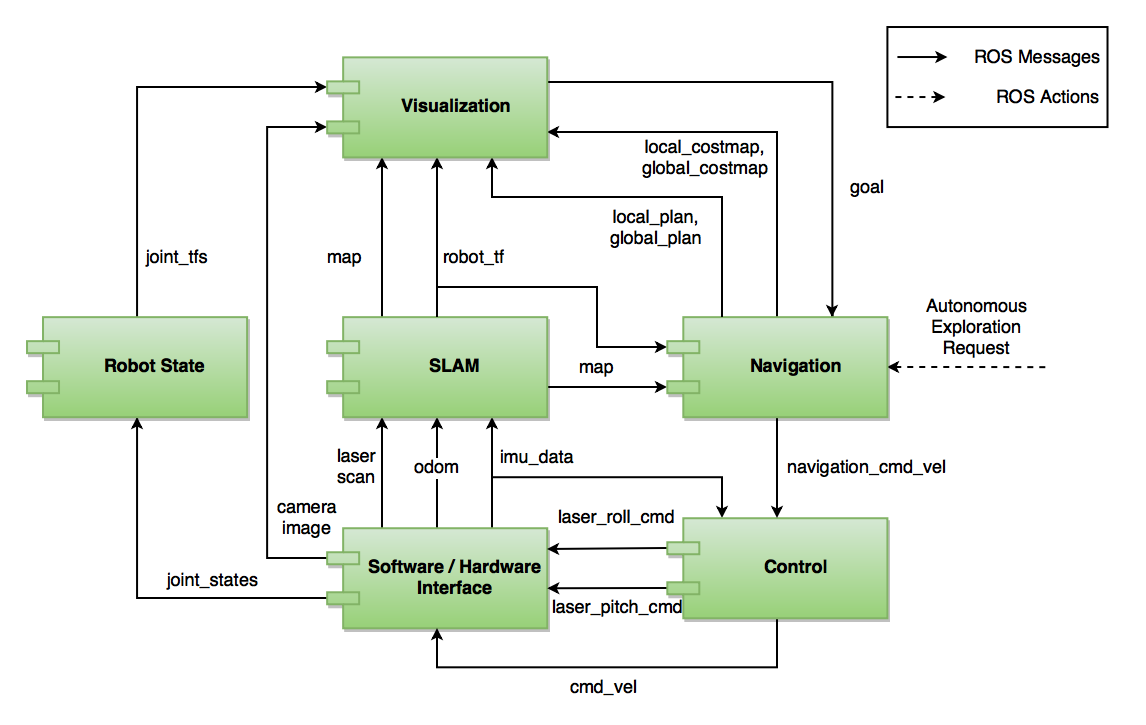
\includegraphics[width=\linewidth]{Chapters/Chapter4/Figures/component_diagram.png}
	\caption{Το διάγραμμα τμημάτων του λογισμικού της ρομποτικής πλατφόρμας Monstertruck.}
	\label{fig:component_diagram}
\end{figure}

\bigskip
Κάθε τμήμα του λογισμικού που παρουσιάζεται στο σχήμα \ref{fig:component_diagram} αποτελείται από ένα σύνολο κόμβων, συμβατών με το ROS και υπεύθυνων για τις λειτουργίες που απαιτούνται από το αντίστοιχο τμήμα, όπως παρουσιάζεται στη συνέχεια.

\subsection{Software/Hardware Interface} \label{ssec:sw_hw_interface_component}
Το τμήμα του \textit{Software/Hardware Interface} αποτελεί ένα επίπεδο διεπαφής των επιμέρους περιφερειακών συσκευών του ρομπότ με το framework του ROS. Η δομή, η οποία χρησιμοποιείται στο λογισμικό της ομάδας P.A.N.D.O.R.A για έναν κόμβο Software/Hardware Interface αποτελείται βασικά από τον driver της συσκευής, συνήθως ανεξάρτητο από το ROS, που επιτρέπει την επικοινωνία μεταξύ του υπολογιστή και της συσκευής, μέσω ενός πρωτοκόλλου  σειριακής επικοινωνίας, έναν wrapper που αποτελεί την διεπαφή μεταξύ του driver και του ROS και τέλος έναν ROS Controller, ο οποίος αποτελεί ένα plugin που μπορεί να φορτώνεται ή να σταματάει δυναμικά και είναι υπεύθυνο για την έκδοση και την λήψη μετρήσεων και εντολών αντίστοιχα, ως μηνύματα του ROS. Στην συνέχεια παρουσιάζεται το σύνολο των κόμβων του επιπέδου Software/Hardware Interface.

\begin{figure}[!ht]
	\centering
	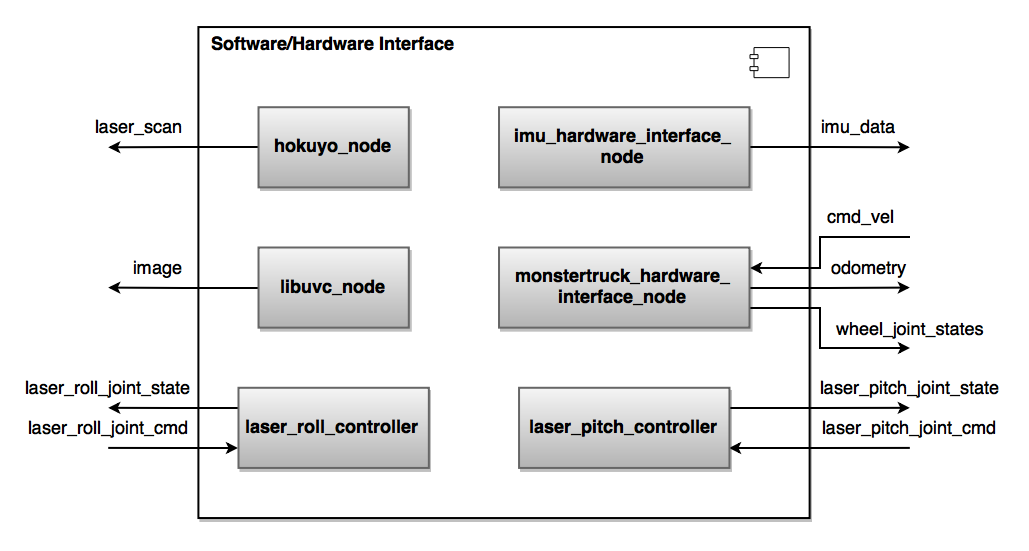
\includegraphics[width=0.8\linewidth]{Chapters/Chapter4/Figures/hardware_component_diagram.png}
	\caption{Το διάγραμμα των κόμβων του τμήματος Software/Hardware Interface της ρομποτικής πλατφόρμας Monstertruck.}
	\label{fig:hardware_component_diagram}
\end{figure}

\begin{itemize}
	\item Ο κόμβος \textbf{hokuyo{\_}node} \cite{hokuyo_node}  είναι υπεύθυνος για την διεπαφή του σαρωτή λέιζερ Hokuyo URG-04LX, με το framework του ROS, εκδίδοντας μηνύματα ROS με τις σαρώσεις του αισθητήρα, όπως επίσης και τις παραμέτρους του (πχ. εμβέλεια, εύρος γωνίας σάρωσης, κλπ).
	\item Οι κόμβοι \textbf{laser{\_}roll{\_}controller} και \textbf{laser{\_}pitch{\_}controller} είναι \textbf{dynamixel{\_}controllers}  \cite{dynamixel_controllers} και είναι υπεύθυνοι για την διεπαφή των έξυπνων σερβοκινητήρων Dynamixel, που χρησιμοποιούνται για την σταθεροποίηση του σαρωτή λέιζερ στο οριζόντιο επίπεδο.
	\item Ο κόμβος \textbf{libuvc{\_}node} του πακέτου \textbf{libuvc{\_}camera} \cite{libuvc} είναι υπεύθυνος για την διεπαφή της κάμερας Logitech C905, λαμβάνοντας εικόνες-frames από αυτήν και έπειτα μεταδίδοντας τις μέσω μηνυμάτων ROS.
	\item Ο κόμβος \textbf{imu{\_}hardware{\_}interface} του πακέτου \textbf{pandora{\_}imu{\_}hardware{\_}interface} είναι υπεύθυνος για την διεπαφή μεταξύ της πυξίδας Compass OS4000 και του ROS, και χρησιμοποιείται για την παροχή του προσανατολισμού του ρομπότ ως προς τους άξονες $x,y,z$, δηλαδή τις μετρήσεις roll, pitch, yaw, όπως επίσης και για τις γραμμικές επιταχύνσεις $a_x,a_y,a_z$. του ρομπότ ως προς τους τρεις άξονες.
	\item Ο κόμβος \textbf{monstertruck{\_}hardware{\_}interface} του πακέτου \textbf{pandora{\_}monstertruck{\_}hardware{\_} interface,} που γράφτηκε στα πλαίσια της παρούσας διπλωματικής εργασίας είναι υπεύθυνος για την διεπαφή του λογισμικού με τον ελεγκτή EPOS 24/1 του κινητήρα του συστήματος τετρακίνησης και με τον ελεγκτή Pololu Micro Maestro των σερβοκινητήρων του συστήματος τετραδιεύθυνσης της ρομποτικής πλατφόρμας Monstertruck. Επομένως, λαμβάνει μηνύματα-εντολές κίνησης του οχήματος, τις μετατρέπει σε εντολές κίνησης του κινητήρα και των σερβοκινητήρων, βάσει της ανάλυσης που προηγήθηκε στην ενότητα \ref{ssec:monstertruck_kinematics} και έπειτα τις προωθεί σ' αυτούς. Παράλληλα, εκδίδει μηνύματα σχετικά με τις μετρήσεις ταχύτητας και θέσης των τροχών.
\end{itemize}

\subsection{Control} \label{ssec:control_component}
Το τμήμα \textit{Control} περιλαμβάνει κόμβους υπεύθυνους για τον μερικό ή ολικό έλεγχο των κινούμενων μερών της ρομποτικής πλατφόρμας Monstertruck. Συγκεκριμένα, περιλαμβάνει τους ακόλουθους κόμβους, όπως παρουσιάζονται και στο σχήμα \ref{fig:control_component_diagram}.

\begin{figure}[!ht]
	\centering
	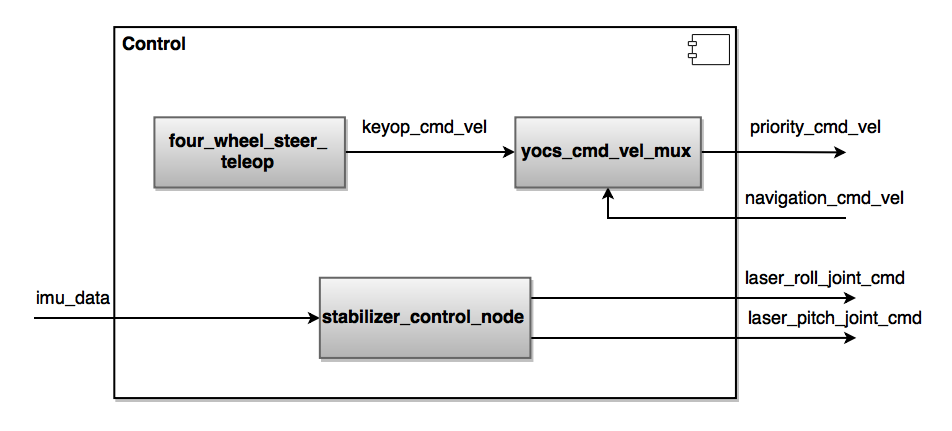
\includegraphics[width=0.8\linewidth]{Chapters/Chapter4/Figures/control_component_diagram.png}
	\caption{Το διάγραμμα των κόμβων του τμήματος Control της ρομποτικής πλατφόρμας Monstertruck.}
	\label{fig:control_component_diagram}
\end{figure}

\begin{itemize}
	\item Ο κόμβος \textbf{stabilizer{\_}control{\_}node} του πακέτου \textbf{pandora{\_}stabilizer} είναι υπεύθυνος για τον έλεγχο θέσης των έξυπνων σερβοκινητήρων Dynamixel, που χρησιμοποιούνται για την σταθεροποίηση του σαρωτή λέιζερ στο οριζόντιο επίπεδο. Συγκεκριμένα, λαμβάνει μηνύματα με πληροφορία για τις κλίσεις roll, pitch του οχήματος, από την πυξίδα και έπειτα στέλνει μηνύματα-εντολές με αντίστροφες κλίσης roll, pitch στους έξυπνους σερβοκινητήρες της ρομποτικής πλατφόρμας Monstertruck με στόχο την αντιστάθμιση των κλίσεων και την διατήρηση του σαρωτή λέιζερ στο οριζόντιο επίπεδο. Η εν λόγω αντιστάθμιση κλίσης είναι απαραίτητη, καθώς ένας αλγόριθμος χαρτογράφησης 2D, όπως αυτοί που εξετάζονται μπορεί να παρερμηνεύσει τις σαρώσεις και να παράγει έναν εσφαλμένο χάρτη.
	\item Για τον τηλεχειρισμό της ρομποτικής πλατφόρμας Monstertruck, αναπτύχθηκε ο κόμβος τηλεχειρισμού \textit{four{\_}wheel{\_}steer{\_}teleop}, ο οποίος επιτρέπει τον έλεγχο του οχήματος με βάση το κινηματικό τετραδιεύθυνσης \ref{ssec:4ws_kinematics}, δίνοντας την δυνατότητα κίνησης και με θετική και με αρνητική τετραδιεύθυνση. Οι δύο παραπάνω κόμβοι τηλεχειρισμού εκδίδουν μηνύματα εντολών, τα οποία λαμβάνονται από τον κόμβο monstertruck{\_}hardware{\_}interface, ο οποίος τις  εκτελεί.	
	\item Ο κόμβος \textbf{yocs{\_}cmd{\_}vel{\_}mux} \cite{yocs_cmd_vel_mux} χρησιμοποιήθηκε σαν διαμεσολαβητής μεταξύ εντολής και εκτέλεσης για την προτεραιοποίηση των πηγών εντολών ταχύτητας. Συγκεκριμένα, ένα αυτόνομο ρομποτικό σύστημα όπως η ρομποτική πλατφόρμα Monstertruck μπορεί να λαμβάνει εντολές ταχύτητας από διάφορες πηγές ταυτόχρονα, όπως ο κόμβος αυτόνομης πλοήγησης, ο κόμβος τηλεχειρισμού, κάποιος κόμβος ελέγχου ασφαλείας κοκ, με αποτέλεσμα να δημιουργείται σύγχυση του ρομπότ και η συμπεριφορά του να καθίσταται απρόβλεπτη. Γι αυτό το λόγο χρησιμοποιείται ο κόμβος yocs{\_}cmd{\_}vel{\_}mux ο οποίος αποτελεί ουσιαστικά έναν πολυπλέκτη εντολών ταχυτήτων με βάση την προτεραιότητα των κόμβων από τους οποίους προέρχονται οι εντολές. Στην προκειμένη περίπτωση παρέχεται υψηλότερη προτεραιότητα για τον κόμβο τηλεχειρισμού από τον κόμβο αυτόνομης πλοήγησης, ούτως ώστε να μπορεί να παρακαμφθεί η αυτόνομη λειτουργία σε περίπτωση κινδύνου ή ανεπιθύμητης συμπεριφοράς.
\end{itemize}

\subsection{SLAM} \label{ssec:slam_components}
Στην ενότητα \ref{sec:localization_and_mapping} παρουσιάστηκαν οι αλγόριθμοι SLAM και οι μέθοδοι εκτίμησης κατάστασης που χρησιμοποιήθηκαν στην ρομποτική πλατφόρμα Monstertruck. Στην παρούσα ενότητα, παρουσιάζονται δύο διαφορετικά τμήματα που μπορούν να χρησιμοποιηθούν για την χαρτογράφηση και την εκτίμηση της θέσης του ρομπότ. Πριν προχωρήσουμε, παρόλα αυτά, στα εν λόγω τμήματα, είναι πολύ σημαντικό για την κατανόηση τους, να ορισθούν τα ακόλουθα \textit{πλαίσια αναφοράς} (\textit{reference frames}), όσον αφορά την παρούσα εφαρμογή.

\begin{itemize}
	\item \textbf{world:} Είναι η ρίζα στο δέντρο των πλαισίων αναφοράς και αποτελεί έναν αμετάβλητο πλαίσιο αναφοράς, που στην προκειμένη περίπτωση επιλέγεται βάσει της αρχικής πόζας του ρομπότ.
	\item \textbf{map:} Είναι ένα σταθερό πλαίσιο αναφοράς ως προς το πλαίσιο world και αναπαριστά την αρχή των αξόνων του χάρτη που παράγεται από έναν αλγόριθμο SLAM. Η πόζα του ρομπότ δεν ολισθαίνει σημαντικά με τον χρόνο, με βάση το πλαίσιο αυτό, αλλά μπορεί να μεταβάλλεται σπασμωδικά.
	\item \textbf{odom:} Είναι ένα σταθερό πλαίσιο αναφοράς ως προς το πλαίσιο map. Είναι ακατάλληλο πλαίσιο αναφοράς για μακροπρόθεσμη καθολική αναφορά, επειδή η πόζα του ρομπότ στο πλαίσιο αυτό μπορεί να ολισθαίνει χωρίς όρια, με την πάροδο του χρόνου, αλλά, παρόλα αυτά, εγγυάται συνεχή και ομαλή μεταβολή της πόζας, χωρίς διακριτές μεταβολές, σε αντίθεση με το πλαίσιο αναφοράς map.
	\item \textbf{base{\_}footprint:} Αποτελεί το πλαίσιο αναφοράς του αποτυπώματος του ρομπότ στο επίπεδο, όσον αφορά το πλαίσιο αναφοράς map ή odom.
	\item \textbf{base{\_}link:} Αποτελεί το πλαίσιο αναφοράς του ρομπότ, λαμβάνοντας υπόψιν την 6D κατάσταση $(x,y,z,yaw,pitch,roll)$ του, όσον αφορά το πλαίσιο αναφοράς base{\_}footprint.
	\item \textbf{laser{\_}link:} Αποτελεί το πλαίσιο αναφοράς του σαρωτή λέιζερ.
\end{itemize}

\bigskip Στην συνέχεια παρουσιάζονται τα δύο διαφορετικά συστήματα χαρτογράφησης και εκτίμησης κατάστασης που εξετάστηκαν στα πλαίσια της παρούσας διπλωματικής εργασίας.

\subsubsection{CRSM-SLAM}
Το πρώτο σύστημα χαρτογράφησης και εκτίμησης κατάστασης που εξετάστηκε αποτελείται από δύο κόμβους, όπως παρουσιάζεται στο σχήμα \ref{fig:slam_1_component_diagram}.

\begin{figure}[!ht]
	\centering
	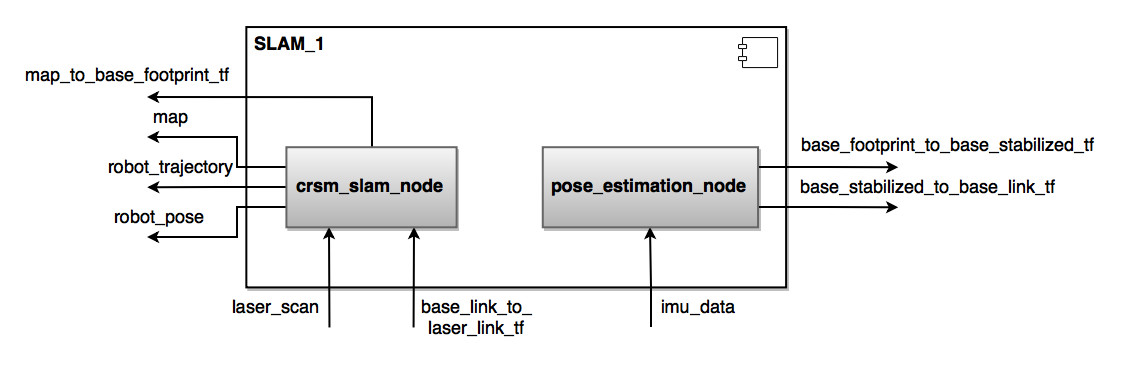
\includegraphics[width=\linewidth]{Chapters/Chapter4/Figures/slam_1_component_diagram.png}
	\caption{Διάγραμμα κόμβων του τμήματος χαρτογράφησης και εκτίμησης κατάστασης, με τον αλγόριθμο CRSM-SLAM.}
	\label{fig:slam_1_component_diagram}
\end{figure}

\begin{itemize}
	\item Ο κόμβος \textbf{crsm{\_}slam{\_}node} του πακέτου \textbf{crsm{\_}slam} \cite{crsm_slam_node} είναι υπεύθυνος για την χαρτογράφηση του περιβάλλοντος του ρομπότ και του ταυτόχρονου εντοπισμού της πόζας του, ως προς τον χάρτη που παράγει. Για την λειτουργία του, ο κόμβος αυτός, απαιτεί μηνύματα τύπου \textit{sensor{\_}msgs/LaserScan} με σαρώσεις του περιβάλλοντος από έναν σαρωτή λέιζερ, όπως ο Hokuyo URG-04LX που χρησιμοποιείται στην ρομποτική πλατφόρμα Monstertruck, όπως επίσης και τον μετασχηματισμό μεταξύ των πλαισίων αναφοράς base{\_}link και laser{\_}link. Με βάση αυτές τις πληροφορίες παράγει έναν 2D χάρτη πλέγματος κατάληψης κελιού (OGM) του περιβάλλοντος, ενώ παράλληλα εκδίδει μέσω μηνυμάτων την πόζα $(x,y,\theta)$ του ρομπότ, την τροχιά που έχει ακολουθήσει από τη στιγμή που ξεκίνησε και τον μετασχηματισμό μεταξύ των πλαισίων αναφοράς map και base{\_}footprint.
	
	\item Ο κόμβος \textbf{pose{\_}estimation{\_}node} του πακέτου \textbf{pandora{\_}pose{\_}estimation} είναι υπεύθυνος για την έκδοση του μετασχηματισμού μεταξύ των πλαισίων αναφοράς base{\_}footprint και base{\_}link, όπου λαμβάνονται υπόψιν οι κλίσεις roll, pitch του ρομπότ, τις οποίες λαμβάνει από τον κόμβο του αισθητήρα Compass OS4000. Επομένως, συμπληρώνεται η κατάσταση του ρομπότ και από τις κλίσεις roll, pitch του ρομπότ, έχοντας ως αποτέλεσμα την εκτίμηση της 5D κατάστασης $(x,y,\theta,roll,pitch)$ του ρομπότ, χωρίς, παρόλα αυτά, να λαμβάνεται υπόψιν η θέση του ρομπότ ως προς τον κατακόρυφο άξονα $z$, λόγω έλλειψης κάποιου αλγόριθμου που να την υπολογίζει με εύρωστο τρόπο.

\end{itemize}

\begin{figure}[!ht]
	\centering
	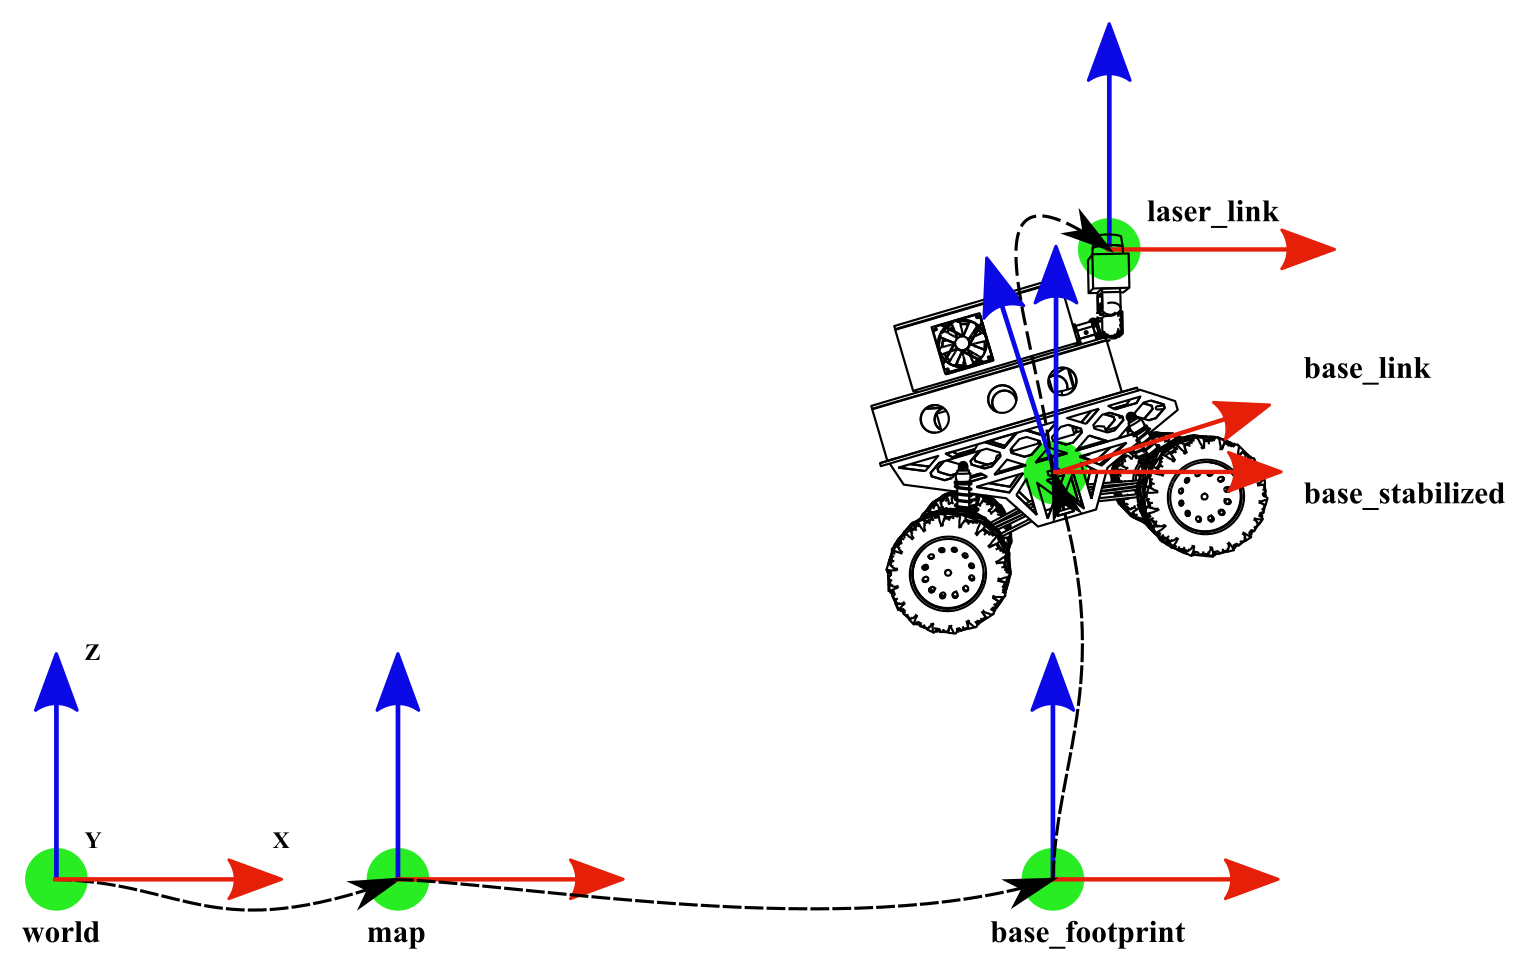
\includegraphics[width=\linewidth]{Chapters/Chapter4/Figures/slam_1_reference_frames.png}
	\caption{Πλαίσια αναφοράς, βάσει του συστήματος χαρτογράφησης και εκτίμησης κατάστασης με τον αλγόριθμο CRSM-SLAM.}
	\label{fig:slam_1_reference_frames}
\end{figure}

\subsubsection{GMapping και State Estimation με EKF}
Το δεύτερο σύστημα χαρτογράφησης και εκτίμησης κατάστασης που εξετάστηκε αποτελείται, επίσης από δύο κόμβους, όπως παρουσιάζεται στο σχήμα \ref{fig:slam_2_component_diagram}.

\begin{figure}[!ht]
	\centering
	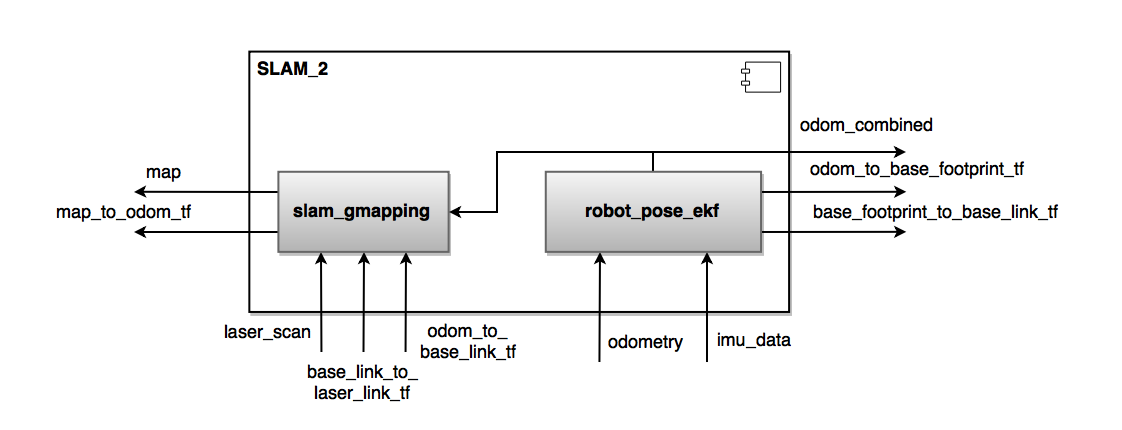
\includegraphics[width=\linewidth]{Chapters/Chapter4/Figures/slam_2_component_diagram.png}
	\caption{Διάγραμμα κόμβων του τμήματος χαρτογράφησης και εκτίμησης κατάστασης, με τον αλγόριθμο GMapping και με EKF.}
	\label{fig:slam_2_component_diagram}
\end{figure}

\begin{itemize}
		\item Ο κόμβος \textbf{slam{\_}gmapping} του πακέτου \textbf{gmapping} \cite{gmapping_package} είναι μία υλοποίηση του αλγορίθμου Gmapping που αναφέρθηκε στην ενότητα \ref{sssec:gmapping}, συμβατή με το ROS. Ο κόμβος αυτός, λαμβάνει σαρώσεις λέιζερ του περιβάλλοντος, την οδομετρία του οχήματος, όπως επίσης και τους μετασχηματισμούς μεταξύ των πλαισίων αναφοράς base{\_}link, laser{\_}link και odom, base{\_}link και δημιουργεί τον χάρτη του περιβάλλοντος, όπως επίσης και τον μετασχηματισμό μεταξύ των πλαισίων αναφοράς map και odom.
		\item Ο κόμβος \textbf{robot{\_}pose{\_}ekf} του πακέτου \textbf{robot{\_}pose{\_}ekf} \cite{robot_pose_ekf} χρησιμοποιεί ένα EKF με ένα 6D μοντέλο (3D θέσης και 3D προσανατολισμός) για να συνδυάσει τις μετρήσεις της οδομετρίας των τροχών και της πυξίδας, ενώ δίνει την δυνατότητα συμπερίληψης και μετρήσεων οπτικής οδομετρίας, με απώτερο στόχο την παραγωγή μίας πιο εύρωστης αντίληψης για την 6D κατάσταση του ρομπότ, σε σύγκριση με εκτιμήσεις από μεμονωμένες πηγές πληροφορίας. Στην προκειμένη περίπτωση, λαμβάνει, μέσω μηνυμάτων ROS, την οδομετρία των τροχών και τις μετρήσεις της πυξίδας και εκδίδει την συνδυασμένη οδομετρία και τους μετασχηματισμούς μεταξύ των πλαισίων αναφοράς odom, base{\_}footprint και base{\_}footprint, base{\_}link.

\end{itemize}

\begin{figure}[!ht]
	\centering
	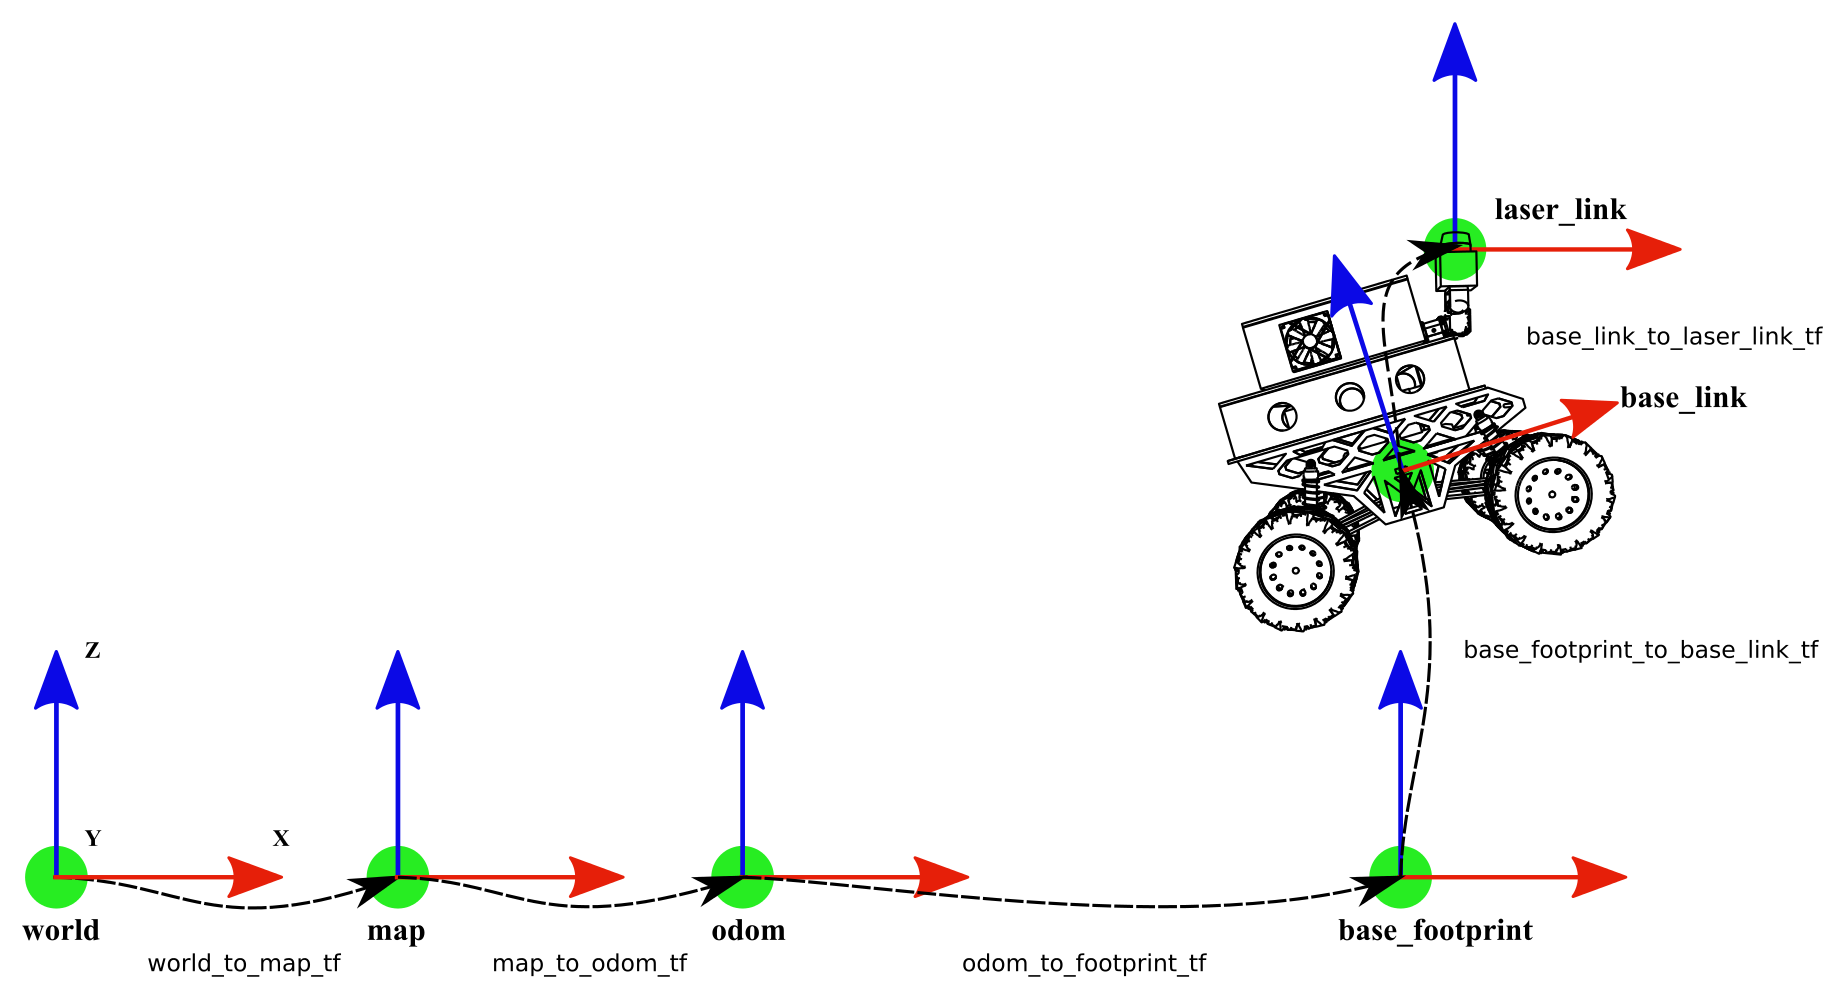
\includegraphics[width=\linewidth]{Chapters/Chapter4/Figures/slam_2_reference_frames.png}
	\caption{Πλαίσια αναφοράς, βάσει του συστήματος χαρτογράφησης και εκτίμησης κατάστασης με τον αλγόριθμο Gmapping και με EKF.}
	\label{fig:slam_2_reference_frames}
\end{figure}

%%%%%%%%%%%%%%%%%%%%%%%%%%%%%%%%%%%%%%%%%%%%%%%%%%%%%%%%%%%%%%%%%%%%%%%%%%%%%%%%%%%%%%%%%%%%%
\subsection{Navigation} \label{ssec:navigation_system_architecture}
Το σύστημα αυτόνομης πλοήγησης της ρομποτικής πλατφόρμας Monstertruck, όπως παρουσιάζεται στο σχήμα \ref{fig:navigation_component_diagram}, αποτελείται, βασικά, από τον κόμβο \textbf{move{\_}base} \cite{move_base}, ο οποίος είναι υπεύθυνος για την πλοήγηση του οχήματος, με στόχο την αυτόνομη μετάβαση του από μία αρχική θέση σε μία τελική, αλλά και έναν προαιρετικό κόμβο \textbf{exploration{\_}controller} του πακέτου \textbf{pandora{\_}explorer} ο οποίος χρησιμοποιείται για την εξερεύνηση του περιβάλλοντος, μέσω της παραγωγής διαδοχικών στόχων, σε αντίθεση με την επιλογή στόχων από τον χειριστή/επόπτη του ρομπότ.

\begin{figure}[!ht]
	\centering
	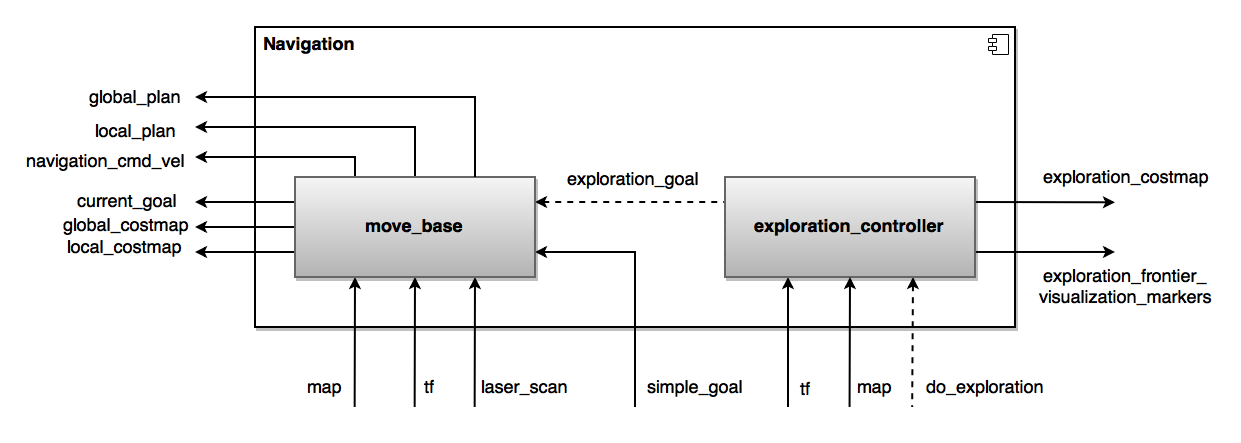
\includegraphics[width=\linewidth]{Chapters/Chapter4/Figures/navigation_component_diagram.png}
	\caption{Το τμήμα αυτόνομης πλοήγησης της ρομποτικής πλατφόρμας Monstertruck.}
	\label{fig:navigation_component_diagram}
\end{figure}

\bigskip
Ο κόμβος \textbf{exploration{\_}controller}, χρησιμοποιεί έναν αλγόριθμο επιλογής στόχων \cite{zalidis_thesis}, με σκοπό την πλήρη εξερεύνηση του περιβάλλοντος. Χρησιμοποιεί σαν είσοδο την τρέχουσα πόζα του ρομπότ και μία αναπαράσταση του περιβάλλοντος, στη προκειμένη περίπτωση τον χάρτη πλέγματος κατάληψης, βάσει των οποίων αναζητά μέτωπα προς εξερεύνηση. Ως μέτωπα εξερεύνησης επιλέγονται τα σύνορα μεταξύ εξερευνημένου και ανεξερεύνητου χώρου, ενώ η επιλογή του τρέχοντος μετώπου εξερεύνησης πραγματοποιείται, λαμβάνοντας υπόψιν διάφορες συναρτήσεις κόστους μετρικών, όπως το μέγεθος του συνόρου, του μήκος του μονοπατιού για μετάβαση στο σύνορο αυτό, την γωνιακή απόκλιση μεταξύ του ρομπότ και του συνόρου και την συχνότητα επιλογής αυτού.

\bigskip
Ο κόμβος \textbf{move{\_}base} αποτελεί έναν κόμβο ο οποίος, δοσμένου ενός στόχου, προσπαθεί να πλοηγήσει το ρομπότ προς τον στόχο αυτόν. Όπως παρουσιάζεται στο σχήμα \ref{fig:move_base}, αυτό το πετυχαίνει συνδυάζοντας έναν \textit{global{\_}planner} για την κατασκευή ενός ολικού μονοπατιού που βρίσκεται εξ ολοκλήρου στον ελεύθερο χώρο και συνδέει το ρομπότ με τον στόχο και έναν \textit{local{\_}planner} ο οποίος προσπαθεί να ακολουθήσει το ολικό μονοπάτι, αποφεύγοντας ταυτόχρονα τυχόν δυναμικά εμπόδια και γενικότερα απρόβλεπτες καταστάσεις, λαμβάνοντας υπόψιν κινηματικούς και δυναμικούς περιορισμούς του ρομπότ. Ο κόμβος move{\_}base, επίσης, δημιουργεί και διαχειρίζεται δύο \textit{2D χάρτες κόστους} (\textit{costmap{\_}2d}), τον \textit{global{\_}costmap}, που αποτελεί μία αναπαράσταση του ολικού τρέχοντος χάρτη, και χρησιμοποιείται από τον global{\_}planner για την κατασκευή του \textit{ολικού μονοπατιού} (\textit{global{\_}plan}), όπως επίσης και τον \textit{local{\_}costmap}, που αναπαριστά μία τοπική αναπαράσταση του τρέχοντος χάρτη, με κέντρο το ρομπότ, το οποίο χρησιμοποιείται από τον local{\_}planner, για την κατασκευή του \textit{τοπικού μονοπατιού} (\textit{local{\_}plan}). Επίσης, ο κόμβος move{\_}base υποστηρίζει \textit{ρουτίνες επαναφοράς} (\textit{recovery behaviors}) σε περίπτωση που ο global{\_}planner ή ο local{\_}planner αποτύχουν να βρουν μία εφικτή λύση.

\bigskip
Το μεγάλο πλεονέκτημα του κόμβου move{\_}base αποτελεί η ευελιξία του και η προσαρμοστικότητα του, όσον αφορά την δυνατότητα χρήσης διαφορετικών αλγορίθμων για κατασκευή μονοπατιών, αποφυγή εμποδίων, επαναφορά από αποτυχία κοκ, μέσω προσθέτων (plugins), που αποτελεί και έναν τους λόγους που επιλέχθηκε για την υλοποίηση του συστήματος αυτόνομης πλοήγησης της ρομποτικής πλατφόρμας Monstertruck.

\begin{figure}[!ht]
	\centering
	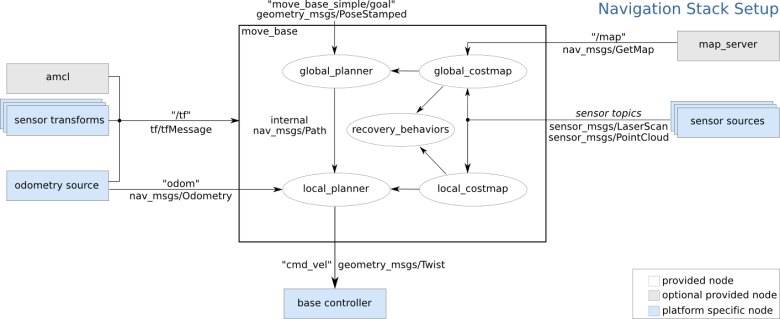
\includegraphics[width=\linewidth]{Chapters/Chapter4/Figures/move_base.png}
	\caption{Ο κόμβος move{\_}base με τις βασικές απαιτούμενες διεπαφές \cite{move_base}.}
	\label{fig:move_base}
\end{figure}

Στην συνέχεια, παρουσιάζονται πιο αναλυτικά οι 2D χάρτες κόστους, οι ρουτίνες επαναφοράς, όπως επίσης και τα δύο συστήματα αυτόνομης πλοήγησης που υλοποιήθηκαν.

\subsubsection{2D Χάρτες Κόστους}
\bigskip
Ο κόμβος move{\_}base, όπως προαναφέρθηκε χρησιμοποιεί 2D χάρτες κόστους \cite{costmap_2d}, οι οποίοι παράγονται, βάσει του χάρτη πλέγματος κατάληψης κελιού ενός αλγορίθμου SLAM και συντίθενται από έναν αριθμό επιπέδων. Στην προκειμένη περίπτωση, χρησιμοποιούνται τρία επίπεδα, όπου το \textit{στατικό επίπεδο} (\textit{static layer}) αναπαριστά τα αμετάβλητα τμήματα ενός χάρτη κόστους, όπως αυτά παράγονται από έναν αλγόριθμο SLAM, το \textit{επίπεδο των εμποδίων} (\textit{obstacle layer}) αναπαριστά τα εμπόδια όπως αυτά αναγνωρίζονται από μετρήσεις του σαρωτή λέιζερ και το \textit{επίπεδο διαστολής} (\textit{inflation layer}) που μεταδίδει τα κόστη ακτινικά των εμποδίων, όπως αναφέρθηκε και στην ενότητα \ref{sec:autonomous_navigation}, προσπαθώντας να μετατρέψει τον χάρτη κόστους στο χώρο εφικτών καταστάσεων του ρομπότ. Στο σχήμα \ref{fig:costmap_inflation_costs} παρουσιάζονται τα διάφορα κόστη ενός χάρτη κόστους, τα οποία ορίζονται ακολούθως, αν λάβουμε το κόστος ως έναν μη προσημασμένο ακέραιο με 8bit.

\begin{itemize}
	\item \textbf{cost{\_}unknown(255)}: Είναι το κόστος των κελιών, για τα οποία δεν είναι γνωστή η κατάσταση κατάληψης.
	\item \textbf{cost{\_}lethal(254)}: Είναι το κόστος των κελιών που ανήκουν σε εμπόδια.
	\item \textbf{cost{\_}inscribed(253)}: Είναι το κόστος των κελιών στα οποία το ρομπότ έρχεται σε σύγκρουση και έχουν απόσταση από τα κελιά των εμποδίων, ίση με την ακτίνα του κύκλου που εγγράφεται στο αποτύπωμα του ρομπότ.
	\item \textbf{cost{\_}possibly{\_}circumscribed(128)}: Είναι το κόστος των κελιών που η απόσταση τους από τα κελιά των εμποδίων ισούται με την ακτίνα του περιγεγραμμένου, στο αποτύπωμα του ρομπότ, κύκλου. Κόστη που ανήκουν στο διάστημα $[128, 252]$ δηλώνουν πιθανή σύγκρουση που καθορίζεται από τον προσανατολισμό του ρομπότ.
	\item \textbf{cost{\_}safe $\in [128,0)$}: Κόστος κελιών που μπορούν να προσπελαστούν από το ρομπότ χωρίς κίνδυνο για σύγκρουση. Η απόσταση τους από τα κελιά των εμποδίων μπορεί να οριστεί από τον χρήστη. 
	\item \textbf{cost{\_}freespace (0)}: Είναι το κόστος των ελεύθερων κελιών που δεν εισάγουν κανένα περιορισμό προσπέλασης από το ρομπότ και θα πρέπει γενικά να προτιμάται, κατά την κατασκευή μονοπατιών και την πλοήγηση του ρομπότ.
\end{itemize}

\begin{figure}[!ht]
	\centering
	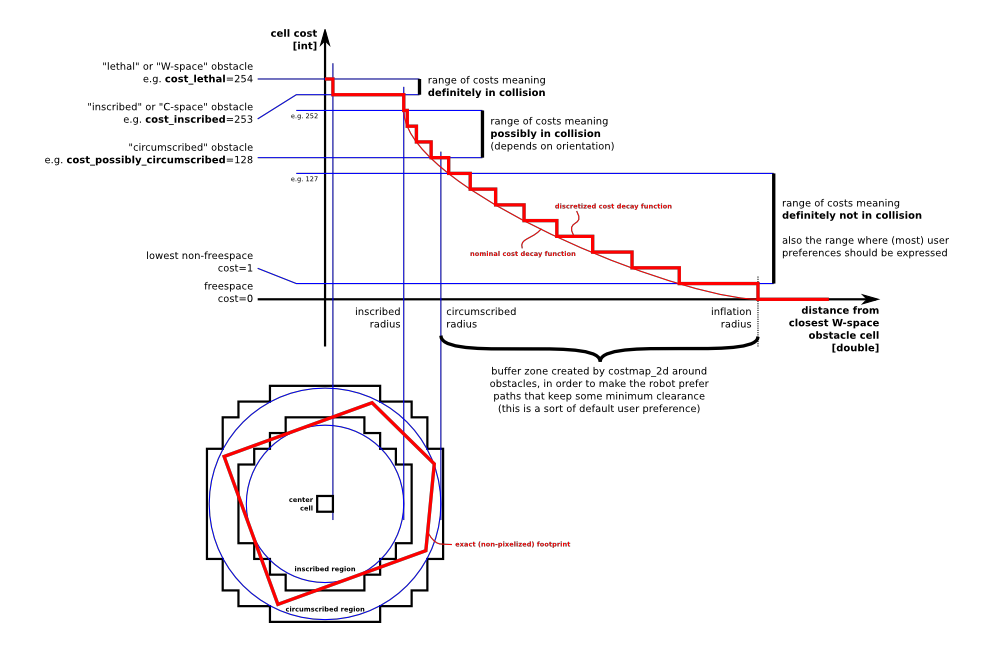
\includegraphics[width=\linewidth]{Chapters/Chapter4/Figures/costmap_inflation_costs.png}
	\caption{Τα κόστη του επιπέδου διαστολής του 2D χάρτη κόστους \cite{costmap_2d}.}
	\label{fig:costmap_inflation_costs}
\end{figure}


\begin{figure}[!ht]
	\centering
	\subfloat[OGM.]{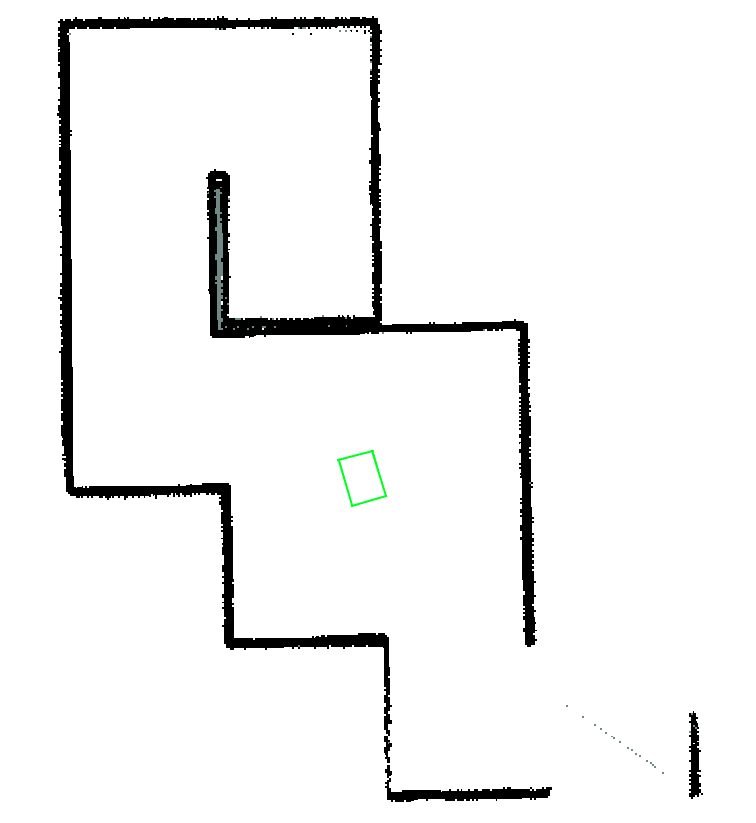
\includegraphics[height=5cm]{Chapters/Chapter4/Figures/map.png}}
	\subfloat[Global Costmap.]{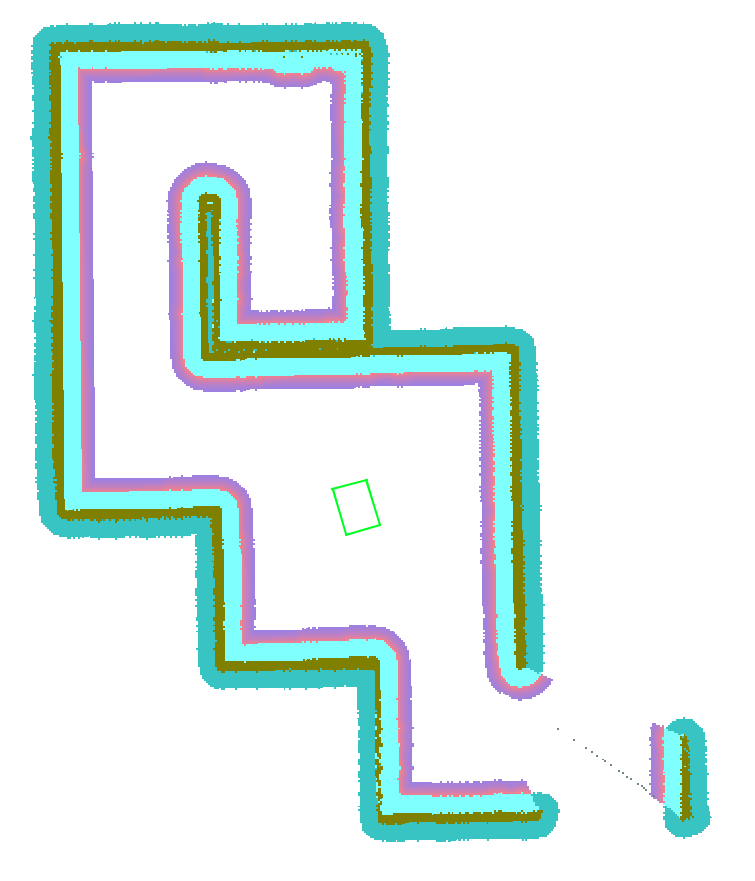
\includegraphics[height=5cm]{Chapters/Chapter4/Figures/global_costmap.png}}
	\subfloat[Local Costmap.]{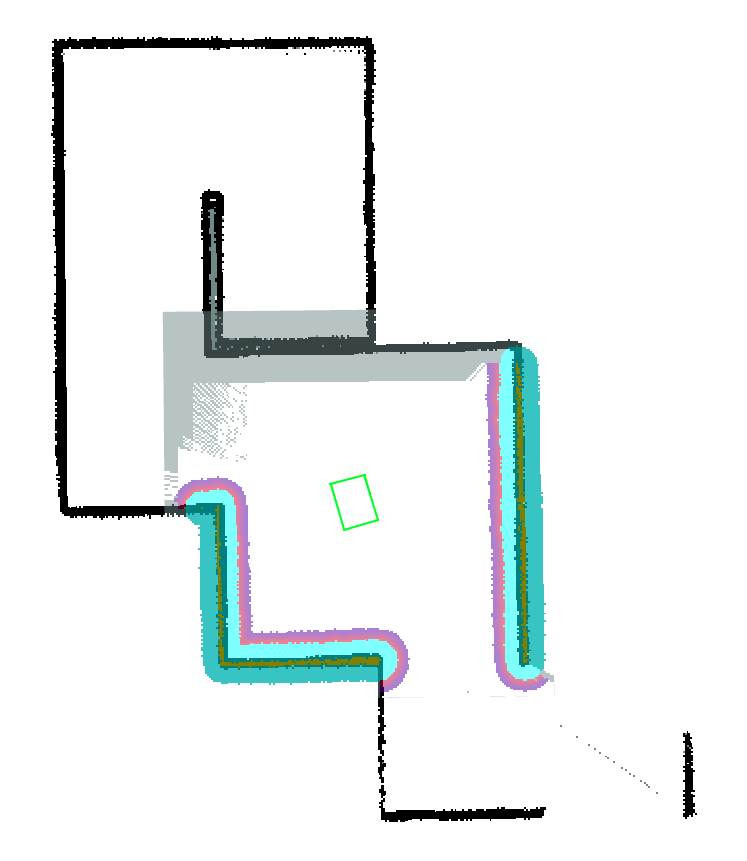
\includegraphics[height=5cm]{Chapters/Chapter4/Figures/local_costmap.png}}
	\caption{Ο χάρτης πλέγματος κατάληψης κελιού που παράχθηκε από τον αλγόριθμο CRSM-SLAM, για το περιβάλλον robocup του προσομοιωτή STDR και οι αντίστοιχοι χάρτες κόστους.}
	\label{fig:costmaps}
\end{figure}


\subsubsection{Ρουτίνες Επαναφοράς}
Ένα πολύ σημαντικό τμήμα του κόμβου move{\_}base αποτελεί μία ακολουθία ρουτινών επαναφοράς που εκτελούνται σε περίπτωση που το ρομπότ έχει κολλήσει, δηλαδή έχει αποτύχει ο global{\_}planner ή ο local{\_}planner να παράξουν κάποιο μονοπάτι ή τροχιά για την επίτευξη του τρέχοντα στόχου. Οι ρουτίνες επαναφοράς στοχεύουν στον καθαρισμό του χώρου περιμετρικά του ρομπότ, έτσι ώστε να μπορεί να ξεκολλήσει. Αρχικά, λοιπόν, πραγματοποιείται καθαρισμός των εμποδίων έξω από μία περιοχή γύρω από το ρομπότ, που ορίζεται αυθαίρετα. Έπειτα, ακολουθεί μία επιτόπου περιστροφή του ρομπότ με στόχο τον καθαρισμό τυχόν εσφαλμένων εμποδίων ή άγνωστου χώρου που εμφανίζονται στον χάρτη κόστους. Αν η ρουτίνα αυτή αποτύχει, τότε επαναλαμβάνεται η διαδικασία, αλλά για την ελάχιστη δυνατή περιοχή που επιτρέπει την επί τόπου περιστροφή του ρομπότ. Εάν, παρόλα αυτά, και αυτή η ρουτίνα αποτύχει, τότε ο στόχος ορίζεται σαν μη εφικτός.

\bigskip
Όπως είναι προφανές, η παραπάνω ακολουθία ρουτινών επαναφοράς δεν είναι εφικτές για ένα μη ολονομικό όχημα, που δεν μπορεί να πραγματοποιήσει επί τόπου στροφές, όπως για παράδειγμα η υλοποιημένη ρομποτική πλατφόρμα Monstertruck. Επομένως, επιλέχθηκε η ανάπτυξη μίας ρουτίνας επαναφοράς που προσπαθεί να ξεφύγει από ανεπιθύμητες καταστάσεις, πραγματοποιώντας κινηματικά εφικτούς ελιγμούς.

\bigskip
Η κυριότερη αιτία αποτυχίας κατασκευής ολικού ή τοπικού μονοπατιού, αποτελεί συνήθως η πολύ κοντινή απόσταση του ρομπότ σε εμπόδια. Για το λόγο αυτό, αναπτύχθηκε η ρουτίνα επαναφοράς \textbf{car{\_}maneuver{\_}recovery} που προσπαθεί μέσω κινηματικά εφικτών ελιγμών να απομακρύνει το ρομπότ από εμπόδια. Η εν λόγω ρουτίνα επαναφοράς υποστηρίζει κινήσεις, βάσει κινηματικού Ackermann, θετικής τετραδιεύθυνσης και αρνητικής τετραδιεύθυνσης και λειτουργεί όπως παρουσιάζεται στον Αλγόριθμο~\ref{alg:car_maneuver_recovery}

\newpage
\begin{algorithm}[!ht]
	\caption{Αλγόριθμος Ρουτίνας Επαναφοράς car{\_}maneuver{\_}recovery}
	\label{alg:car_maneuver_recovery}
	\textbf{Input:} frontSideCost, rearSideCost, leftSideCost, rightSideCost, fourWheelSteering, crabSteering\\
	\textbf{Output:} speed, frontSteeringAngle, rearSteeringAngle
	\begin{algorithmic}[1]
		\State front $\leftarrow$ frontSideCost < COST{\_}POSSIBLY{\_}CIRCUMSCRIBED
		\State rear  $\leftarrow$ rearSideCost < COST{\_}POSSIBLY{\_}CIRCUMSCRIBED
		\State left  $\leftarrow$ leftSideCost < COST{\_}POSSIBLY{\_}CIRCUMSCRIBED
		\State right $\leftarrow$ rightSideCost < COST{\_}POSSIBLY{\_}CIRCUMSCRIBED
		\If{front \&\& right}
			\If	{frontSideCost > rearSideCost}
				\State speed $\leftarrow$ recoverySpeed
			\Else
				\State speed $\leftarrow$ -recoverySpeed
			\EndIf
		\Else
			\State speed $\leftarrow$ (front - rear) $\times$ recoverySpeed
		\EndIf
		\State frontSteeringAngle $\leftarrow$ (left-right) $\times$ recoverySteeringAngle
		\If {fourWheelSteering}	\Comment Four Wheel Steering
			\If {crabSteering} \Comment Positive Four Wheel Steering
				\State rearSteeringAngle $\leftarrow$ frontSteeringAngle
			\Else \Comment Negative Four Wheel Steering
				\State rearSteeringAngle $\leftarrow$ - frontSteeringAngle
			\EndIf
		\Else \Comment Ackermann Steering
			\State rearSteeringAngle $\leftarrow$ 0
		\EndIf
	\end{algorithmic}
\end{algorithm}

\bigskip
\noindent
όπου τα κόστη frontSideCost, rearSideCost, leftSideCost και rightSideCost υπολογίζονται ως ο μέσος όρος των κοστών της αντίστοιχης πλευράς του αποτυπώματος του ρομπότ στον τοπικό χάρτη κόστους και οι μεταβλητές fourWheelSteering και crabSteering δηλώνουν την προτίμηση του χρήστη για τον ελιγμό που θα πραγματοποιεί η ρουτίνα επαναφοράς.

\begin{figure}[!ht]
	\centering
	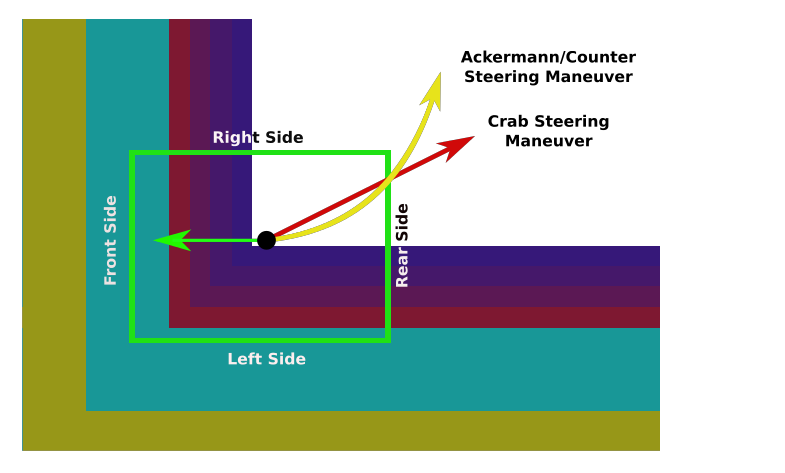
\includegraphics[height=6cm]{Chapters/Chapter4/Figures/car_maneuver_recovery_example.png}
	\caption{Παράδειγμα εκτέλεσης ρουτίνας επαναφοράς του αλγορίθμου car{\_}maneuver{\_}recovery.}
	\label{fig:car_maneuver_recovery_example}
\end{figure}


\bigskip
Στην συνέχεια, παρουσιάζονται τα δύο συστήματα αυτόνομης πλοήγησης που χρησιμοποιήθηκαν, με βάση τον κόμβο move{\_}base, τα οποία διαφοροποιούνται όσον αφορά την αρχιτεκτονική και την συνολική προσέγγιση επίλυσης του προβλήματος, μέσω της επιλογής διαφορετικών ζευγών αλγορίθμων local{\_}planner και global{\_}planner.
	
\subsubsection{Σύστημα Αυτόνομης Πλοήγησης με Δυναμική Παραμόρφωση Μονοπατιού (DPM)}
Το πρώτο σύστημα αυτόνομης πλοήγησης που υλοποιήθηκε με βάση τον κόμβο move{\_}base, αποτελείται από έναν global planner ο οποίος κατασκευάζει ένα στατικό ολικό μονοπάτι στον ελεύθερο χώρο του ολικού χάρτη κόστους (global costmap), βάσει των αλγορίθμων A* ή Dijkstra και από έναν local planner που παίρνει το ολικό μονοπάτι και παραμορφώνει δυναμικά (Dynamic Path Modification) το τμήμα αυτού που ανήκει στον τοπικό χάρτη κόστους με στόχο την παραγωγή ενός τοπικού, κινηματικά εφικτού και ασφαλούς μονοπατιού, βάσει του αλγορίθμου Reeds-Shepp Band, που παρουσιάστηκε στην ενότητα \ref{sssec:rsband}.

\begin{figure}[!ht]
	\centering
	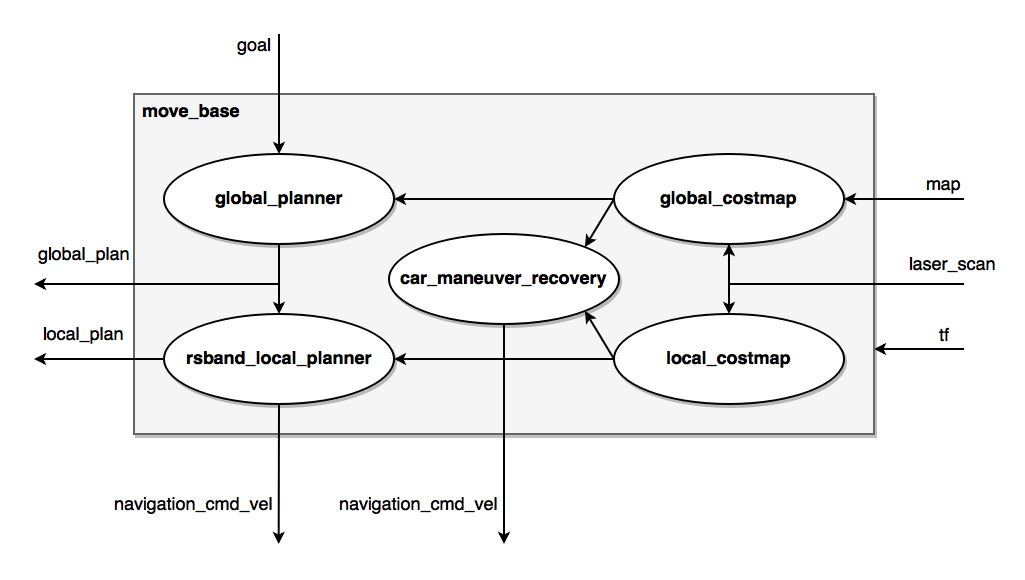
\includegraphics[width=\linewidth]{Chapters/Chapter4/Figures/navigation_1_plugins.png}
	\caption{Ο κόμβος move{\_}base με τα plugins του συστήματος αυτόνομης πλοήγησης με δυναμική παραμόρφωση μονοπατιού.}
	\label{fig:navigation_1_plugins}
\end{figure}

\begin{itemize}
	\item Το plugin \textbf{global{\_}planner} του \citeauthor{global_planner} \cite{global_planner} είναι ένα plugin του κόμβου move{\_}base, το οποίο υλοποιεί τους αλγορίθμους αναζήτησης μονοπατιού A* και Dijkstra που αναφέρθηκαν στην ενότητα \ref{ssec:path_planning}, με στόχο την εύρεση ενός μονοπατιού που βρίσκεται εξ ολοκλήρου στον ελεύθερο χώρο του ολικού χάρτη κόστους και ενώνει την αρχική θέση του ρομπότ με τον στόχο.
	\item Το plugin \textbf{rsband{\_}local{\_}planner}, που αναπτύχθηκε στα πλαίσια της παρούσας διπλωματικής εργασίας, υλοποιεί τον αλγόριθμο Reeds-Shepp Band, που παρουσιάστηκε στην ενότητα \ref{ssec:obstacle_avoidance}, σε συνδυασμό με τον ελεγκτή διάσχισης μονοπατιού ασαφούς λογικής που παρουσιάστηκε στην ενότητα \ref{ssec:path_following}. Για την υλοποίηση του εν λόγω αλγορίθμου χρησιμοποιήθηκε η υλοποίηση του αλγορίθμου ελαστικής ζώνης των \citeauthor{eband_local_planner} \cite{eband_local_planner} και η υλοποίηση του χώρου καταστάσεων Reeds-Shepp (Reeds-Shepp State Space) του \citeauthor{reeds_shepp_ompl} \cite{reeds_shepp_ompl} της βιβλιοθήκης OMPL (Open Motion Planning Library) \cite{ompl}. Επίσης, για την ανάπτυξη του αλγορίθμου διάσχισης μονοπατιού, που βασίζεται σε ασαφή λογική, χρησιμοποιήθηκε η βιβλιοθήκη ελέγχου ασαφούς λογικής fuzzylite \cite{fuzzylite} του \citeauthor{fuzzylite}. Στο σχήμα \ref{fig:rsband_activity_diagram} παρουσιάζεται η βασική λειτουργικότητα του plugin rsband{\_}local{\_}planner, μέσω ενός προσεγγιστικού διαγράμματος δραστηριοτήτων.
\end{itemize}

\begin{figure}[!ht]
	\centering
	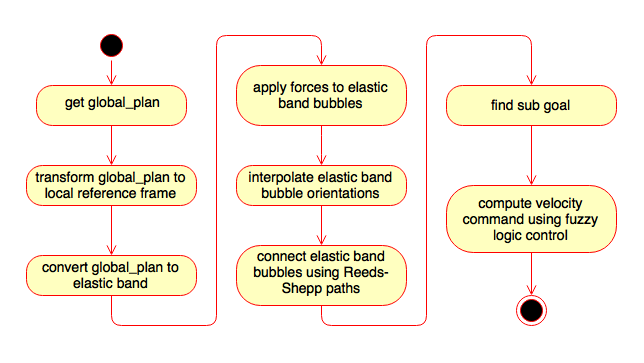
\includegraphics[width=0.7\linewidth]{Chapters/Chapter4/Figures/rsband_activity_diagram.png}
	\caption{Το διάγραμμα δραστηριοτήτων του plugin rsband{\_}local{\_}planner.}
	\label{fig:rsband_activity_diagram}
\end{figure}

\subsubsection{Σύστημα Αυτόνομης Πλοήγησης με Δυναμική Ανακατασκευή Μονοπατιού (DPR)}
Το δεύτερο σύστημα αυτόνομης πλοήγησης που υλοποιήθηκε, με βάση τον κόμβο move{\_}base χρησιμοποιεί έναν global planner για την κατασκευή ενός ολικού κινηματικά εφικτού μονοπατιού με δυναμική ανακατασκευή (Dynamic Path Replanning), αλλά και έναν local planner που απλά χρησιμοποιείται για την διάσχιση του ολικού μονοπατιού.

\begin{figure}[!ht]
	\centering
	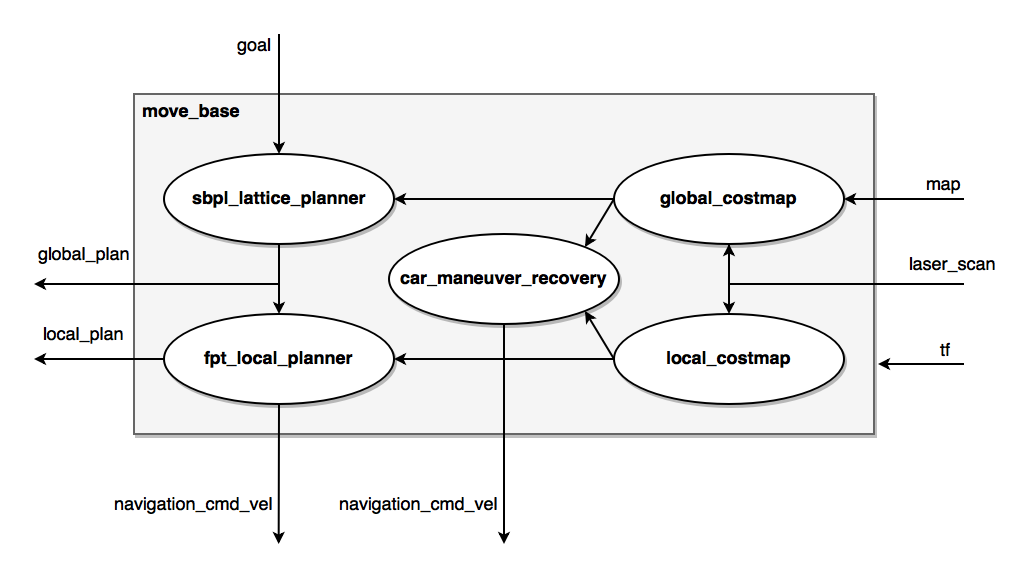
\includegraphics[width=\linewidth]{Chapters/Chapter4/Figures/navigation_2_plugins.png}
	\caption{Ο κόμβος move{\_}base με τα plugins του συστήματος αυτόνομης πλοήγησης με δυναμική ανακατασκευή μονοπατιού.}
	\label{fig:navigation_2_plugins}
\end{figure}

\begin{itemize}
	\item Για την κατασκευή του ολικού μονοπατιού του συστήματος αυτόνομης πλοήγησης με δυναμική ανακατασκευή μονοπατιού χρησιμοποιείται το plugin \textbf{sbpl{\_}lattice{\_}planner} , το οποίο αναπτύχθηκε από τον \citeauthor{sbpl_lattice_planner}\cite{sbpl_lattice_planner} και βασίζεται στην βιλβιοθήκη SBPL \cite{sbpl_library} του Search-Based Planning Lab. Όπως, παρουσιάστηκε και στην ενότητα \ref{sssec:sbpl}, ο αλγόριθμος παράγει ένα μονοπάτι που αποτελείται από τον συνδυασμό ενός συνόλου βασικών κινήσεων (motion primitives), οι οποίες αποτελούν μικρές κινηματικά εφικτές κινήσεις. Η κατασκευή του μονοπατιού, πραγματοποιείται μέσω των αλγορίθμων $ARA*$ ή $AD*$ στον χώρο $(x,y,\theta)$ και επομένως λαμβάνει υπόψιν τον προσανατολισμό του ρομπότ, σε αντίθεση με το σύστημα αυτόνομης πλοήγησης με δυναμική παραμόρφωση μονοπατιού, όπου η αναζήτηση γίνεται στον χώρο $(x,y)$.

\begin{figure}[!ht]
	\centering
	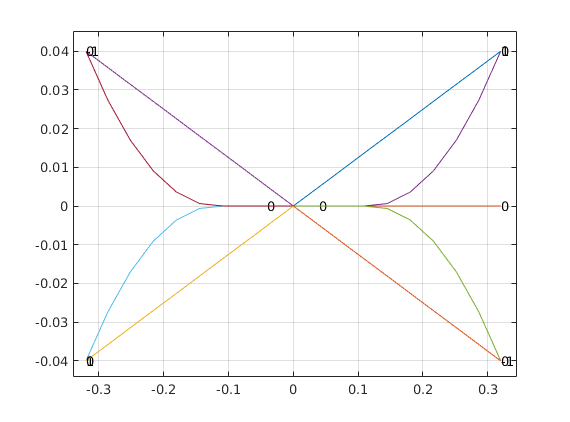
\includegraphics[width=0.6\linewidth]{Chapters/Chapter4/Figures/motion_primitives.png}
	\caption{Οι βασικές κινήσεις που ορίστηκαν για χρήση στον sbpl{\_}lattice{\_}planner, για την κατασκευή μονοπατιών της ρομποτικής πλατφόρμας Monstertruck.}
	\label{fig:motion_primitives}
\end{figure}
		
	\item Αφού κατασκευαστεί το κινηματικά εφικτό ολικό μονοπάτι, με βάση τον παραπάνω αλγόριθμο, χρησιμοποιείται το plugin \textbf{fpt{\_}local{\_}planner}, ως o local{\_}planner του κόμβου move{\_}base, ο οποίος υλοποιεί τον ασαφή ελεγκτή διάσχισης μονοπατιού που παρουσιάστηκε στην ενότητα \ref{ssec:path_following}. Ο ασαφής ελεγκτής δεν πραγματοποιεί αποφυγή εμποδίων, αλλά απλή διάσχιση μονοπατιού και επομένως, η αποφυγή εμποδίων επιτυγχάνεται μέσω της δυναμικής ανακατασκευής του ολικού μονοπατιού.
\end{itemize}


\subsection{Robot State} \label{ssec:robot_state}
Το τμήμα του Robot State αποτελείται από τον κόμβο robot{\_}state{\_}publisher \cite{robot_state_publisher}, ο οποίος χρησιμοποιεί το κινηματικό μοντέλο του ρομπότ, το οποίο φορτώνεται από τον διακομιστή παραμέτρων (parameter server) και βάσει των θέσεων των κινούμενων αρθρώσεων του ρομπότ υπολογίζει και εκδίδει τους μετασχηματισμούς μεταξύ όλων των αρθρώσεων, στατικών και δυναμικών. Για την λειτουργία του, απαιτεί την περιγραφή του μοντέλου του ρομπότ σε μορφή URDF (Unified Robot Description Format), όπως επίσης και κόμβους που εκδίδουν τις θέσεις των κινούμενων αρθρώσεων του.

\begin{figure}[!ht]
	\centering
	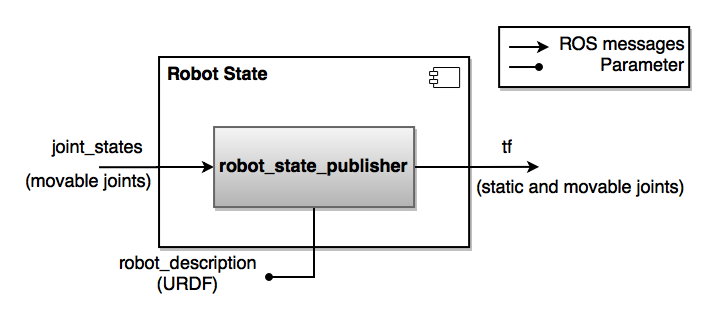
\includegraphics[width=0.7\linewidth]{Chapters/Chapter4/Figures/robot_state_component.png}
	\caption{Το τμήμα Robot State της ρομποτικής πλατφόρμας Monstertruck.}
	\label{fig:robot_state_component}
\end{figure}

\bigskip
Μέσω του URDF είναι δυνατόν να μοντελοποιηθεί ένα ρομπότ σαν ένα σύνολο άκαμπτων συνδέσμων και αρθρώσεων μεταξύ των συνδέσμων αυτών, σε τοπολογία με δενδρική δομή που απαγορεύει κλειστούς βρόχους. Παρόλα αυτά, προσφέρει δυνατότητες για κινηματική και δυναμική περιγραφή του ρομπότ, οπτική αναπαράσταση των συνδέσμων του, όπως επίσης και περιγραφή του μοντέλου σύγκρουσης αυτών.

\bigskip
Στα πλαίσια της παρούσας εργασίας, αναπτύχθηκε ένα λεπτομερές αλλά προσεγγιστικό οπτικά και διαστασιολογικά μοντέλο της ρομποτικής πλατφόρμας Monstertruck σε μορφή URDF. Αρχικά, πραγματοποιήθηκε η ανάπτυξη ενός τρισδιάστατου στατικού μοντέλου, μέσω του προγράμματος \textit{Blender}\footnote{\url{www.blender.org}} και έπειτα, βάσει αυτού αναπτύχθηκε το αντίστοιχο μοντέλο σε μορφή URDF, όπου συμπεριλήφθηκαν και οι αρθρώσεις του ρομπότ. Συνολικά ορίστηκαν δεκαοκτώ κινούμενες αρθρώσεις, όπως αυτές παρουσιάζονται στον πίνακα \ref{tab:joints}.

\begin{table}[!ht]
	\centering
	\captionof{table}{Οι αρθρώσεις του μοντέλου URDF της ρομποτικής πλατφόρμας Monstertruck.}
	\label{tab:joints}
	\begin{tabular}{| l | c | c | c |}
		\hline
	   \textbf{Αρθρώσεις} & \textbf{Τύπος} & \textbf{Όρια} & \textbf{Πλήθος}  \\ \hline
	   άρθρωση ώθησης τροχού & περιστροφική & - & 4 \\ \hline
	   άρθρωση στρέψης τροχού & περιστροφική & $[-25^o, 25^o]$ & 4 \\ \hline
	   ανάρτηση τροχού & πρισματική & $[-0.1, 0.3]$ & 4 \\ \hline 
	   εικονική άρθρωση άξονα τροχών & περιστροφική & $[-10^o, 10^o]$ & 2 \\ \hline
	   εικονική ανάρτηση άξονα τροχών & πρισματική & $[-0.1, 0.3]$ & 2 \\ \hline
		άρθρωση roll σαρωτή λέιζερ & περιστροφική & $[-30^o, 30^o]$ & 1 \\ \hline
		άρθρωση pitch σαρωτή λέιζερ & περιστροφική & $[-30^o, 30^o]$ & 1 \\ \hline
	\end{tabular}
\end{table}

\begin{figure}[!ht]
	\subfloat[]{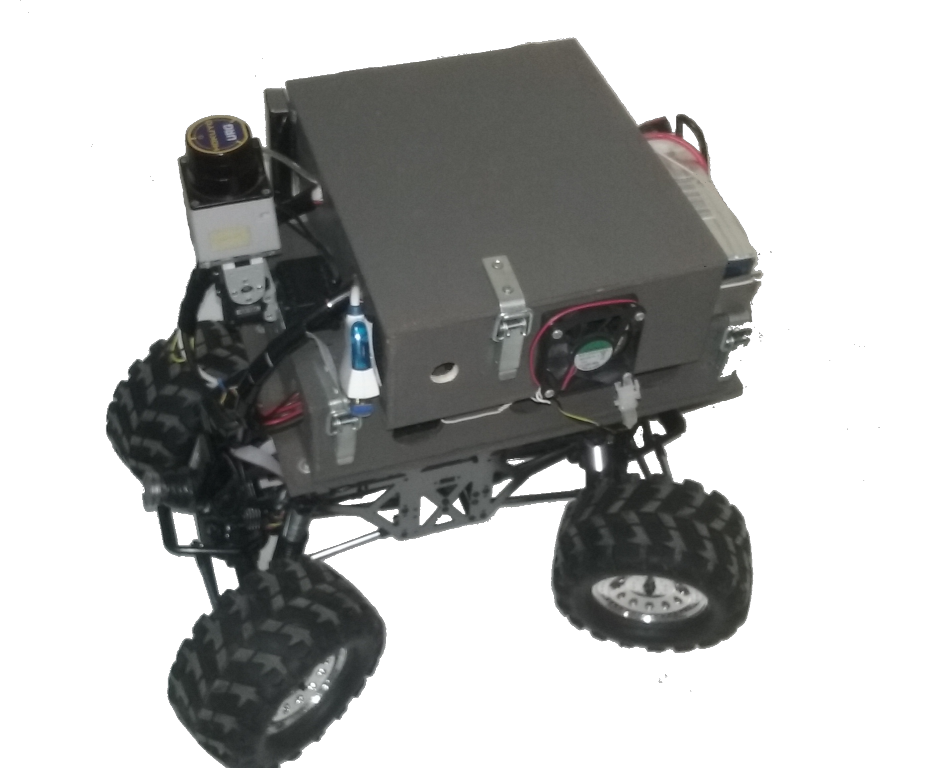
\includegraphics[width=0.33\linewidth]{Chapters/Chapter4/Figures/monstertruck_real.png}}
	\subfloat[]{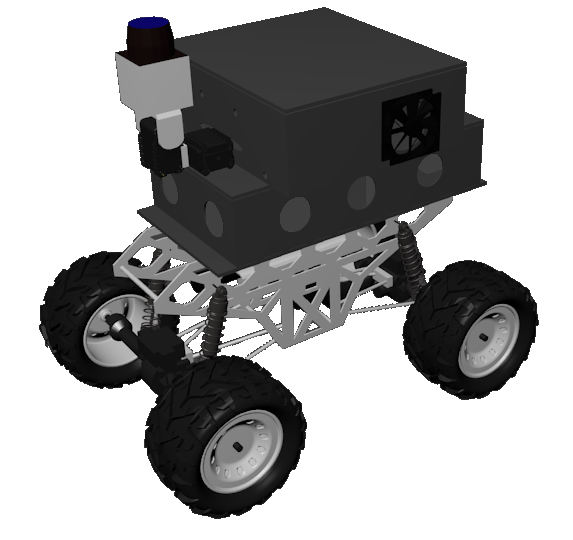
\includegraphics[width=0.33\linewidth]{Chapters/Chapter4/Figures/monstertruck_blender.png}}
	\subfloat[]{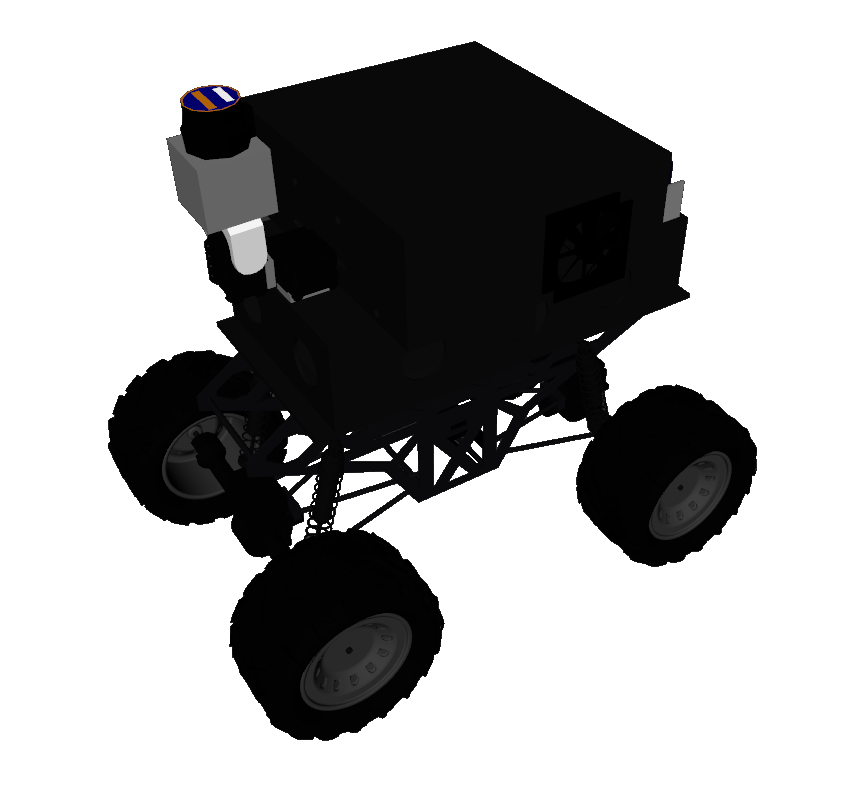
\includegraphics[width=0.33\linewidth]{Chapters/Chapter4/Figures/monstertruck_urdf.png}}
	\caption{Η ρομποτική πλατφόρμα Monstertruck σε (α')φωτογραφία, (β')3D μοντέλο και (γ')URDF.}
	\label{fig:real_model_urdf}
\end{figure}

\bigskip
Η θέση και η ταχύτητα  των αρθρώσεων ώθησης και στρέψης των τροχών, όπως επίσης και των αρθρώσεων σταθεροποίησης του σαρωτή λέιζερ παρέχονται από τους αντίστοιχους κόμβους του τμήματος Software/Hardware Interface \ref{ssec:sw_hw_interface_component}. Παρόλα αυτά, οι αρθρώσεις των αναρτήσεων και των αξόνων των μπροστινών και πίσω τροχών, μοντελοποιήθηκαν για την πιο ρεαλιστική προσομοίωση του ρομπότ, αλλά δεν έχουν καμία χρησιμότητα στο πραγματικό ρομπότ, καθώς δεν υπάρχει κάποιος τρόπος μέτρησης της θέσης τους. Για την προσομοίωση, παρόλα αυτά, η μοντελοποίηση τους πραγματοποιήθηκε με κάποιες προσεγγίσεις. Συγκεκριμένα, η μοντελοποίηση των αναρτήσεων του ρομπότ προσεγγίστηκε μέσω πρισματικών αρθρώσεων με πεπερασμένα όρια δυνάμεων επιβολής της προκαθορισμένης θέσης τους, με αποτέλεσμα, όταν ασκούνται μεγαλύτερες δυνάμεις να ισορροπούν σε διαφορετική θέση. Επίσης, εφόσον το μοντέλο ορίζεται σε δενδρική δομή, που απαγορεύει βρόχους, η κίνηση του μπροστινού και του πίσω άξονα των τροχών προσεγγίσθηκε χρησιμοποιώντας πρισματικές αρθρώσεις για τις κατακόρυφες κινήσεις των αξόνων σε συνδυασμό με περιστροφικές αρθρώσεις για την περιστροφή τους, συναρτήσει της κίνησης των αναρτήσεων των τροχών. 


\begin{figure}[!ht]
	\centering
	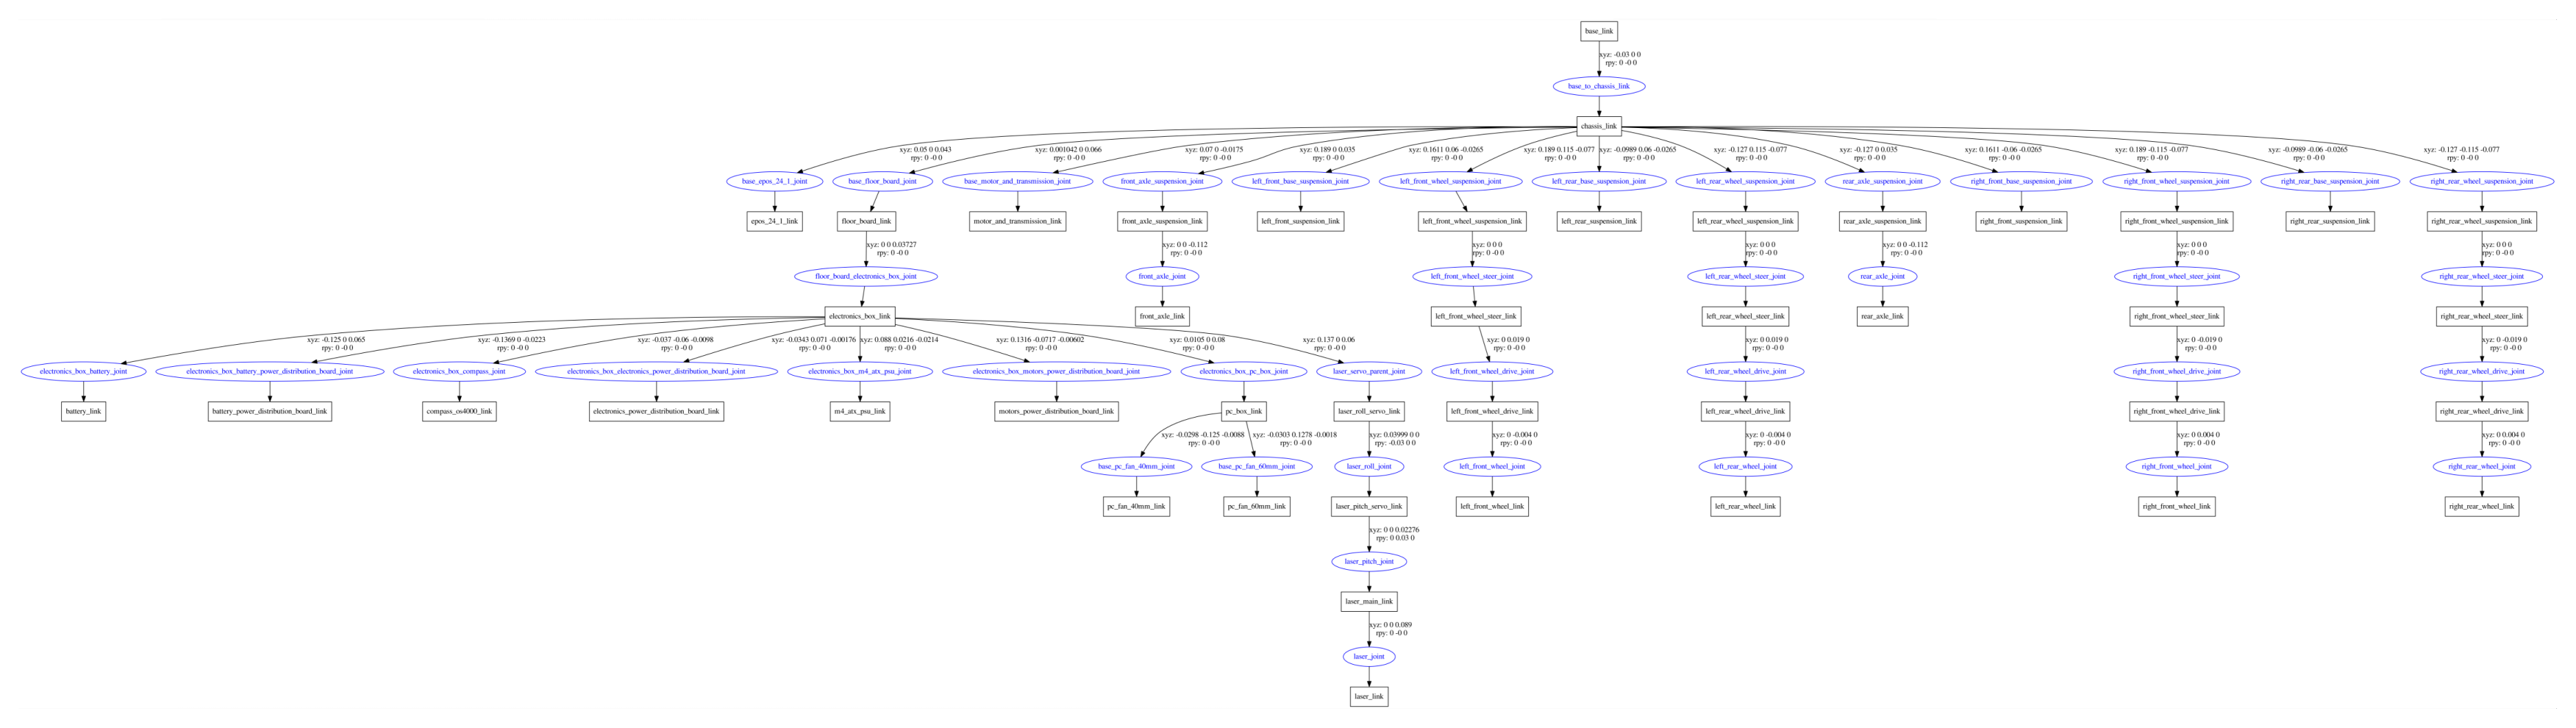
\includegraphics[width=\linewidth]{Chapters/Chapter4/Figures/monstertruck_urdf_tree.png}
	\caption{Πλήρης δενδρική δομή των συνδέσμων και αρθρώσεων της ρομποτικής πλατφόρμας Monstertruck.}
	\label{fig:full_model}
\end{figure}

\begin{figure}[!ht]
	\centering
	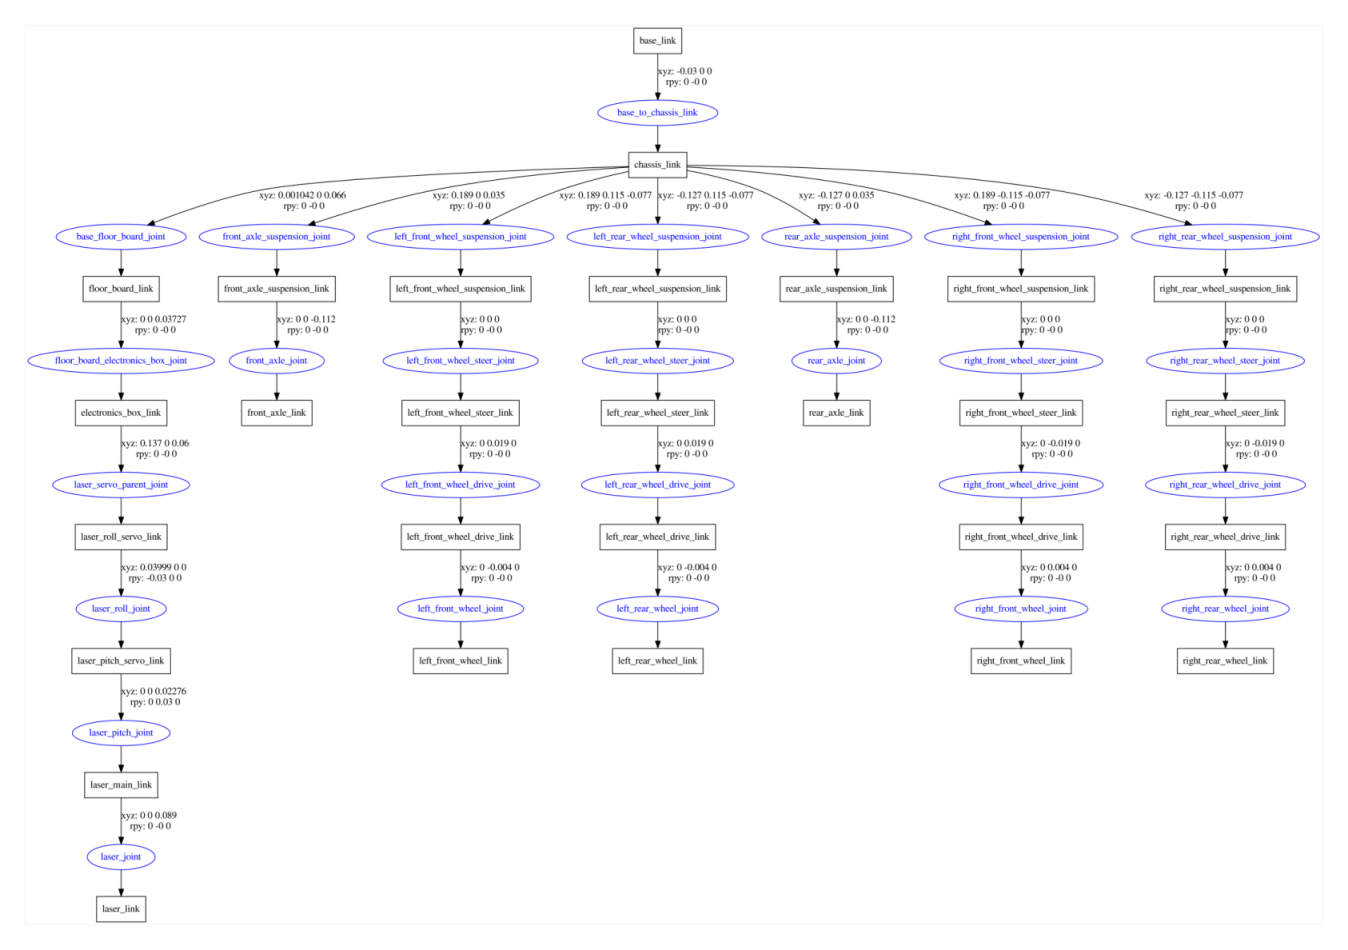
\includegraphics[width=\linewidth]{Chapters/Chapter4/Figures/monstertruck_simplified_urdf_tree.png}
	\caption{Μερική δενδρική δομή των σημαντικότερων συνδέσμων και αρθρώσεων της ρομποτικής πλατφόρμας Monstertruck.}
	\label{fig:simple_model}
\end{figure}


\subsection{Visualization}
Το τμήμα Visualization της ρομποτικής πλατφόρμας Monstertruck αποτελείται από τον κόμβο \textbf{rviz} \cite{rviz}, ο οποίος αποτελεί ένα εργαλείο τρισδιάστατης απεικόνισης για το ROS, με στόχο την απεικόνιση δεδομένων του ρομπότ, όπως μετρήσεις αισθητήρων, χάρτες, το μοντέλου URDF του ρομπότ, ολικά και τοπικά μονοπάτια, στόχους, τροχιά του ρομπότ, εικόνα από κάμερα κοκ, με αποτέλεσμα την δυνατότητα οπτικής επίβλεψης και εντοπισμού προβλημάτων κατά την ανάπτυξη του λογισμικού του ρομπότ, αλλά και κατά την λειτουργία αυτού.

\begin{figure}[!ht]
	\centering
	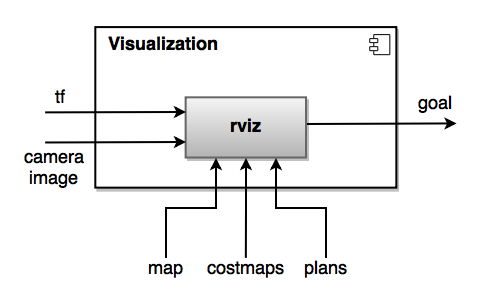
\includegraphics[width=0.5\linewidth]{Chapters/Chapter4/Figures/visualization_component.png}
	\caption{Το τμήμα Visualization της ρομποτικής πλατφόρμας Monstertruck.}
	\label{fig:visualization_component}
\end{figure}


\begin{figure}[!ht]
	\centering
	\frame{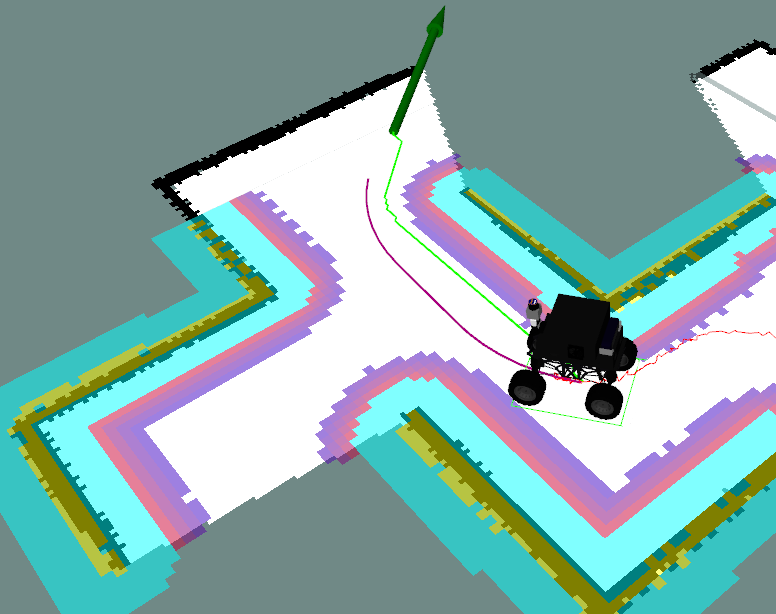
\includegraphics[width=0.45\linewidth]{Chapters/Chapter4/Figures/rviz.png}}
	\caption{Περιβάλλον τρισδιάστατης απεικόνισης από τον κόμβο rviz, όπου παρουσιάζεται το μοντέλο του ρομπότ, ο χάρτης, οι χάρτες κόστους, ο στόχος (πράσινο βέλος) το ολικό μονοπάτι(πράσινο), το τοπικό μονοπάτι(μωβ) και η τρέχουσα τροχιά που έχει διασχιστεί(κόκκινο).}
	\label{fig:rviz}
\end{figure}


%----------------------------------------------------------------------------------------
%	SECTION 3: Simulation Tools
%----------------------------------------------------------------------------------------
\section{Εργαλεία Προσομοίωσης} \label{sec:simulation_tools}
Η ανάπτυξη αλγορίθμων και εφαρμογών για ρομποτικά συστήματα αποτελεί μία ιδιαίτερα σύνθετη, χρονοβόρα και απαιτητική διαδικασία που καθίσταται ακόμα πιο δύσκολη εάν υπάρχει έλλειψη των απαραίτητων εργαλείων και εξοπλισμού ή εάν χρησιμοποιούνται φυσικά συστήματα, τα οποία απαιτούν συνεχή παρακολούθηση και συντήρηση, τα οποία παράλληλα μπορεί να είναι επιρρεπής σε ζημιές. Για παράδειγμα, η ανάπτυξη εφαρμογών αυτόνομης πλοήγησης για ρομποτικά οχήματα, μπορεί να αποτελέσει αρκετά επικίνδυνη διαδικασία, για το ίδιο το ρομπότ και τον εξοπλισμό του, αλλά και για το φυσικό περιβάλλον του, σε περίπτωση εσφαλμένης συμπεριφοράς των αλγορίθμων, περιορίζοντας έτσι σημαντικά τα περιθώρια δυνατών δοκιμών, πάνω σε αυτό. Επίσης, η ανάπτυξη των εφαρμογών απαιτεί συνεχείς δοκιμές πάνω στο ρομπότ και επομένως προϋποθέτει την διαρκή φυσική παρουσία και πλήρη ετοιμότητα αυτού. Τα παραπάνω προβλήματα λύνονται με την χρήση προσομοιωτών ρομποτικών συστημάτων, μέσω των οποίων είναι δυνατή η μοντελοποίηση ενός ή περισσότερων ρομποτικών συστημάτων και η προσομοίωση αυτών, σε ένα τεχνητό περιβάλλον το οποίο μπορεί να αποτελεί μία επαρκής προσέγγιση του πραγματικού περιβάλλοντος, βάσει της εκάστοτε εφαρμογής.

\bigskip
Κατά την ανάπτυξη της ρομποτικής πλατφόρμας Monstertruck, στα πλαίσια της παρούσας διπλωματικής εργασίας, χρησιμοποιήθηκαν δύο προσομοιωτές ρομποτικών συστημάτων, για προσομοίωση του ρομπότ σε δύο και τρεις διαστάσεις, ανάλογα με τις απαιτήσεις του εκάστοτε αντικειμένου, που εξεταζόταν την κάθε στιγμή. Συγκεκριμένα, χρησιμοποιήθηκε ο δισδιάστατος προσομοιωτής \textit{STDR} \cite{stdr} για την προσομοίωση του ρομπότ κατά την ανάπτυξη του συστήματος αυτόνομης πλοήγησης, όσον αφορά την κατασκευή ολικών μονοπατιών, την αποφυγή στατικών εμποδίων, όπως επίσης και την διάσχιση μονοπατιού. Παράλληλα, χρησιμοποιήθηκε ο τρισδιάστατος προσομοιωτής \textit{GAZEBO} \cite{gazebo} κατά την ανάπτυξη του κινηματικού μοντέλου του ρομπότ, όπως επίσης και για την εξέταση της συμπεριφοράς - απόκρισης του συστήματος αυτόνομης πλοήγησης και γενικότερα του συνολικού συστήματος λογισμικού της ρομποτικής πλατφόρμας Monstertruck στις τρεις διαστάσεις, σε προσεγγιστικά πραγματικές συνθήκες, όπως για παράδειγμα ανώμαλο έδαφος. Στην συνέχεια ακολουθεί μία πιο αναλυτική περιγραφή των δύο προσομοιωτών, όπως επίσης και η ενσωμάτωση της ρομποτικής πλατφόρμας Monstertruck στα αντίστοιχα περιβάλλοντα.

\subsection{STDR} \label{ssec:stdr}
Ο προσομοιωτής \textbf{STDR} (Simple Two Dimensional Robot Simulator) αποτελεί έναν απλό, ελαφρύ δισδιάστατο προσομοιωτή, με δυνατότητα ταυτόχρονης προσομοίωσης πολλαπλών ρομπότ. Είναι πλήρως συμβατός με το ROS και στοχεύει στην παροχή μεγάλου πλήθους δυνατοτήτων για ρομποτικές εφαρμογές, χωρίς, παρόλα αυτά, να προσφέρει την πιο ρεαλιστική αναπαράσταση των συνθηκών λειτουργίας του ρομπότ. Ο προσομοιωτής STDR υποστηρίζει ρομπότ με κυκλικό και πολυγωνικό σχήμα, με differential, skid-steer ή omnidirectional κινηματικό μοντέλο, όπως επίσης, μία πληθώρα από αισθητήρες, όπως για παράδειγμα, σαρωτές λέιζερ, αισθητήρες υπερήχων, θερμικούς αισθητήρες, αισθητήρες μέτρησης του διοξειδίου του άνθρακα στο περιβάλλον κ.α. 

\bigskip
Για την προσομοίωση της ρομποτικής πλατφόρμας Monstertruck με τον προσομοιωτή STDR ορίστηκε ένα ρομποτικό μοντέλο με ορθογωνικό αποτύπωμα με τις διαστάσεις του αποτυπώματος του πραγματικού ρομπότ. Όσον αφορά τους αισθητήρες του μοντέλου, χρησιμοποιήθηκε μόνο ένας σαρωτής λέιζερ με αντίστοιχες προδιαγραφές με τον σαρωτή λέιζερ Hokuyo URG-04LX  (πίνακας \ref{tab:hokuyo_specs}), που χρησιμοποιείται στο πραγματικό ρομπότ.

\bigskip
Εφόσον, ο προσομοιωτής STDR δεν υποστηρίζει το κινηματικό μοντέλο τετραδιεύθυνσης που χρησιμοποιεί η ρομποτική πλατφόρμα Monstertruck, χρησιμοποιήθηκε προσεγγιστικά το omnidirectional κινηματικό μοντέλο, σε συνδυασμό με έναν κόμβο που φιλτράρει τις εντολές ταχυτήτων και επιτρέπει μόνο αυτές που είναι εφικτές για το κινηματικό μοντέλο τετραδιεύθυνσης, προσεγγίζοντας έτσι το μοντέλο της ρομποτικής πλατφόρμας Monstertruck.

\begin{figure}[!ht]
	\centering
	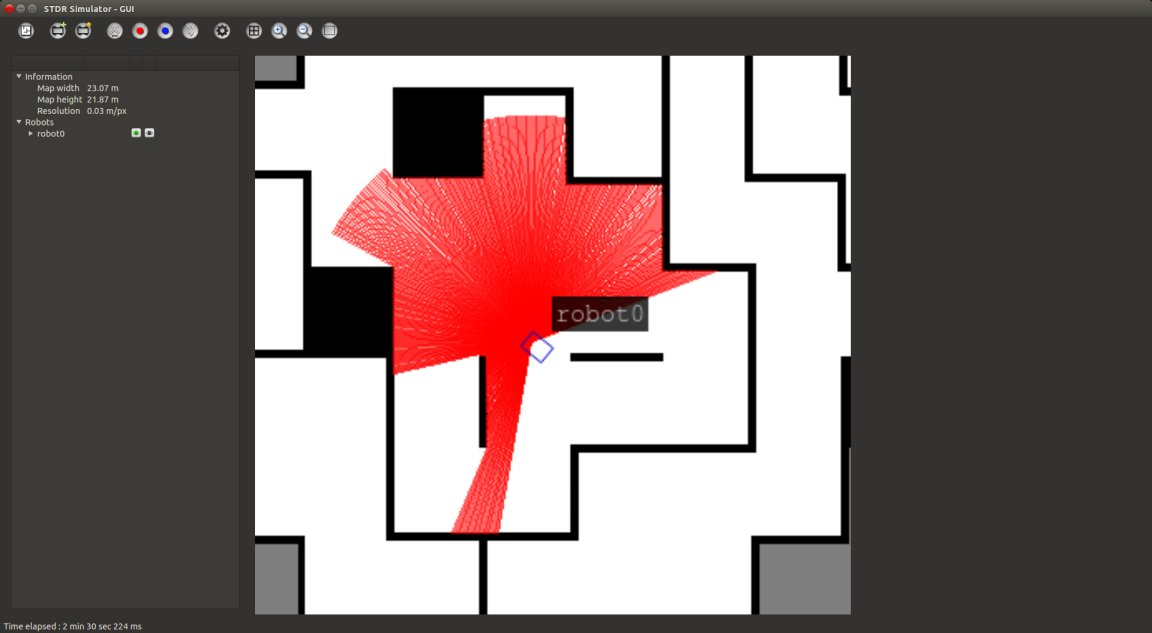
\includegraphics[width=0.7\linewidth]{Chapters/Chapter4/Figures/stdr_simulator.jpg}
	\caption{Περιβάλλον προσομοιωτή STDR.}
	\label{fig:stdr_simulator}
\end{figure}

\FloatBarrier

\subsection{Gazebo} \label{ssec:gazebo}
Το \textbf{Gazebo} αποτελεί έναν τρισδιάστατο προσομοιωτή ρομποτικών συστημάτων, με δυνατότητες ταυτόχρονης προσομοίωσης πολλαπλών ρομπότ, σε εσωτερικά και εξωτερικά δυναμικά περιβάλλοντα μέσω ανεπτυγμένων μηχανών φυσικής. Προσφέρει μία μεγάλη γκάμα ρομποτικών μοντέλων, μοντέλων αισθητήρων και περιβαλλόντων, αλλά και δυνατότητες εύκολης ανάπτυξης και επέκτασης νέων. Σε αντίθεση με δισδιάστατους προσομοιωτές, όπως ο STDR, το Gazebo προσφέρει ένα ιδιαίτερα ρεαλιστικό περιβάλλον για την προσομοίωση ρομποτικών συστημάτων σε συνθήκες αρκετά κοντά στην πραγματικότητα. Συγκεκριμένα, δίνει την δυνατότητα για προσομοίωση ρομποτικών συστημάτων υπό συνθήκες τριβών και ολίσθησης, σε ποικιλόμορφα περιβάλλοντα και αποτελεί ιδανική λύση για ταχεία και ασφαλή δοκιμή αλγορίθμων, όπως επίσης και για ανάπτυξη και προτυποποίηση νέων ρομποτικών συστημάτων.

\bigskip
Στα πλαίσια της παρούσας διπλωματικής εργασίας, ο προσομοιωτής Gazebo χρησιμοποιήθηκε, αρχικά, για την ανάπτυξη και επαλήθευση του κινηματικού μοντέλου της ρομποτικής πλατφόρμας Monstertruck, υπό συνθήκες τριβών και ολίσθησης και έπειτα για την προσομοίωση του πλήρους ρομποτικού συστήματος σε ένα τρισδιάστατο περιβάλλον, με συνθήκες αντίστοιχες, με αυτές για τις οποίες προορίστηκε το πραγματικό ρομπότ, αποφεύγοντας έτσι να τεθεί σε κίνδυνο το φυσικό ρομπότ, πριν επαληθευτεί η εύρωστη συμπεριφορά του συστήματος.

\bigskip
Για την προσομοίωση της ρομποτικής πλατφόρμας Monstertruck χρησιμοποιήθηκε το μοντέλο URDF που αναφέρθηκε στην ενότητα \ref{ssec:robot_state} σε συνδυασμό με ένα σύνολο από plugins για την προσομοίωση της κίνησης των αρθρώσεων του και την λειτουργία των αισθητήρων του, δηλαδή του σαρωτή λέιζερ και της πυξίδας, βάσει των προδιαγραφών του πραγματικού ρομπότ. Επίσης, χρησιμοποιήθηκε και ένα plugin που εκδίδει την ιδανική οδομετρία του ρομπότ για σύγκριση με το μη ιδανικό σύστημα οδομετρίας που αναπτύχθηκε.

\bigskip
\begin{figure}[!ht]
	\centering
	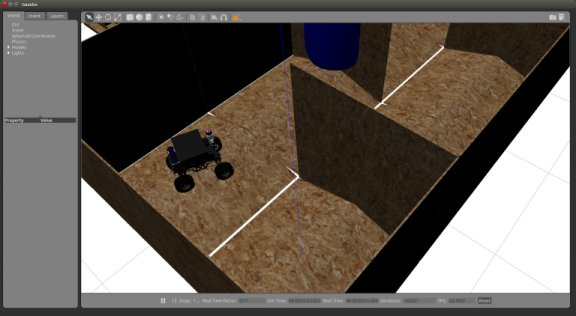
\includegraphics[width=0.7\linewidth]{Chapters/Chapter4/Figures/gazebo_simulator.jpg}
	\caption{Περιβάλλον προσομοιωτή Gazebo.}
	\label{fig:gazebo_simulator}
\end{figure}


%\begin{figure}[!ht]
%	\centering
%	\includegraphics[width=\linewidth]{Chapters/Chapter4/Figures/.png}
%	\caption{}
%	\label{fig:}
%\end{figure}